% !TeX TXS-program:bibliography = txs:///biber
% =====================================================================
%  ВЫПУСКНАЯ КВАЛИФИКАЦИОННАЯ РАБОТА
%  Сборка из материалов преддипломной практики (praktika.tex)
%  и научно-исследовательской работы (vkr.tex).
% =====================================================================
\documentclass[14pt, russian]{scrartcl}
\include{header.tex}
\addbibresource{biblio_vkr.bib}
\usepackage{fvextra}

% Монохромное (чёрно-белое) оформление листингов: без цветовой подсветки.
\usemintedstyle{bw}

\begin{document}
\sloppy

\def\figurename{Рисунок}

% Сквозная нумерация листингов: псевдокод (окружение algorithm, по header
% именуется <<Листинг>>) и код (minted в окружении listing) делят один счётчик,
% чтобы номера <<Листинг N>> не дублировались (требование нормоконтроля).
\makeatletter
\let\c@algorithm\c@listing
\makeatother

% =====================================================================
%  ТИТУЛЬНЫЙ ЛИСТ
% =====================================================================
\begin{titlepage}
\thispagestyle{empty}
\newpage

\bmstuheader

\vspace{3em}

\begin{center}
  \Large \bf{РАСЧЁТНО-ПОЯСНИТЕЛЬНАЯ ЗАПИСКА\\
  \textbf{\textit{К ВЫПУСКНОЙ КВАЛИФИКАЦИОННОЙ РАБОТЕ\\НА ТЕМУ:}}\\}
\end{center}

\vspace*{-6ex}
\begin{center}
  \Large{\textit{\textbf{<<Анализ свойств строковых образцов,\\
  содержащих повторные переменные>>}}}

  \vspace*{-3ex}
  \rule{1\textwidth}{1.2pt}
  \vspace*{-0.2ex}\rule{1\textwidth}{1.2pt}
  \vspace*{-0.2ex}\rule{1\textwidth}{1.2pt}
  \vspace*{-0.2ex}\rule{1\textwidth}{1.2pt}
  \vspace*{-0.2ex}\rule{1\textwidth}{1.2pt}
\end{center}

\vspace{\fill}

\newlength{\ML}
\settowidth{\ML}{«\underline{\hspace{0.7cm}}» \underline{\hspace{2cm}}}

\noindent Студент \underline{\hspace{1.5cm}} \hfill
\underline{\hspace{4cm}}\quad\underline{\hspace{4cm}}

\vspace{-2.1ex}
\noindent\hspace{9ex}\scriptsize{(Группа)}\normalsize\hspace{170pt}
\hspace{2ex}\scriptsize{(Подпись, дата)}\normalsize\hspace{30pt}
\hspace{6ex}\scriptsize{(И.\,О. Фамилия)}\normalsize

\bigskip

\noindent Руководитель ВКР \hfill
\underline{\hspace{4cm}}\quad\underline{\hspace{4cm}}

\vspace{-2ex}
\noindent\hspace{13.5ex}\normalsize\hspace{170pt}
\hspace{2ex}\scriptsize{(Подпись, дата)}\normalsize\hspace{30pt}
\hspace{6ex}\scriptsize{(И.\,О. Фамилия)}\normalsize

\bigskip

\noindent Консультант \hfill
\underline{\hspace{4cm}}\quad\underline{\hspace{4cm}}

\vspace{-2ex}
\noindent\hspace{13.5ex}\normalsize\hspace{170pt}
\hspace{2ex}\scriptsize{(Подпись, дата)}\normalsize\hspace{30pt}
\hspace{6ex}\scriptsize{(И.\,О. Фамилия)}\normalsize

\bigskip

\noindent Нормоконтролёр \hfill
\underline{\hspace{4cm}}\quad\underline{\hspace{4cm}}

\vspace{-2ex}
\noindent\hspace{13.5ex}\normalsize\hspace{170pt}
\hspace{2ex}\scriptsize{(Подпись, дата)}\normalsize\hspace{30pt}
\hspace{6ex}\scriptsize{(И.\,О. Фамилия)}\normalsize

\vfill

\begin{center}
  \textsl{\the\year{} г.}
\end{center}
\end{titlepage}

% =====================================================================
%  АННОТАЦИЯ
% =====================================================================
\setlength{\tabcolsep}{3pt}
\newpage
\setcounter{page}{2}

\section*{АННОТАЦИЯ}

Записка состоит из~\pageref{TotPages} страниц, содержит \totalsections{} разделов,
\totallistings{} листингов, \totaltables{} таблиц и \totalfigures{} рисунков.
Работа посвящена анализу свойств строковых образцов, содержащих повторные
переменные, и разработке оптимизированной эвристики нильсеновского разбиения
для SMT-решателя Ostrich. Предложен и обоснован алгоритм нормализации уравнений
на основе классов коммутации переменных, а также реализовано расширение модуля
\texttt{OstrichNielsenSplitter}, устраняющее избыточное ветвление при обработке
уравнений с удвоенными нетерминалами.

% =====================================================================
%  СОДЕРЖАНИЕ
% =====================================================================
\newpage
\renewcommand\contentsname{\hfill{\normalfont{СОДЕРЖАНИЕ}}\hfill}
\tableofcontents
\newpage

% =====================================================================
%  ВВЕДЕНИЕ
% =====================================================================
\anonsection{ВВЕДЕНИЕ}

Задача проверки выполнимости уравнений в словах (word equations) занимает
центральное место в теоретической информатике и находит широкое применение
в статическом анализе программ, верификации протоколов безопасности и символьном
исполнении кода. Уравнение в словах представляет собой равенство двух слов,
составленных из литералов и переменных, а задача состоит в нахождении такой
подстановки строковых значений вместо переменных, при которой равенство
выполняется. В современной практике анализа программ такие уравнения возникают
при работе с SMT-решателями, поддерживающими теорию строк; среди наиболее
известных решателей этого класса~--- Z3~\cite{demoura2008} и
Ostrich~\cite{chen2022}.

Теоретически значимой задачей в области анализа строковых ограничений является
задача определения однозначности шаблона (pattern ambiguity): по заданному
образцу требуется установить, существует ли строка, соответствующая ему более
чем одним способом. Эта задача сводится к системе строковых ограничений и может
быть передана SMT-решателю, причём эффективность решения критически зависит от
качества эвристик, управляющих разбиением уравнений. Решатель Ostrich реализует
эвристику нильсеновского разбиения, однако в случае уравнений с удвоенными
нетерминалами (паттерн $x^J\cdot y\cdot\Phi_1 = y^I\cdot x\cdot\Phi_2$) базовая
реализация порождает потенциально бесконечное дерево вывода, что делает
актуальной разработку специализированной оптимизации.

\textbf{Целью} настоящей работы является разработка и программная реализация
метода ускоренного отсечения ветвей в алгоритме решения уравнений в словах на
основе обнаружения классов коммутирующих переменных и нормализации уравнений.
Для достижения этой цели изучаются теоретические основы алгоритмов решения
уравнений в словах и эвристики решателей Z3 и Ostrich; анализируется проблема
бесконечного ветвления при обработке повторяющихся переменных; разрабатывается
правило нормализации уравнений на основе классов коммутации с доказательством
его корректности; выполняется реализация обнаружения классов коммутации и
нормализующего преобразования в исходном коде Ostrich, а также проверка
работоспособности модифицированного решателя на задачах однозначности образцов.

\textbf{Объектом исследования} выступает SMT-решатель Ostrich и алгоритм
преобразований Нильсена как его теоретическая основа, а \textbf{предметом}~---
структурные свойства уравнений в словах, порождаемых задачей однозначности
образцов с повторными переменными, и методы ускорения их решения. Практическая
значимость работы состоит в том, что модифицированный решатель способен
обрабатывать более широкий класс образцов за разумное время, что непосредственно
применимо в инструментах статического анализа строковых программ и верификаторах
безопасности.

% =====================================================================
%  РАЗДЕЛ 1. ИССЛЕДОВАТЕЛЬСКАЯ ЧАСТЬ
% =====================================================================
\section{Исследовательская часть}

\subsection{Основные определения}

Пусть $\Sigma$ --- конечный алфавит, $\Sigma^*$ --- множество всех конечных слов над $\Sigma$,
включая пустое слово $\varepsilon$. Множество $\Sigma^*$ образует моноид относительно
операции конкатенации. Пусть $X$ --- счётное множество переменных, $X \cap \Sigma = \varnothing$.
Множество слов над расширенным алфавитом $\Sigma \cup X$ обозначается $(\Sigma \cup X)^*$.

\begin{Definition}
Уравнение в словах над алфавитом $\Sigma$ и множеством переменных $X$ --- это
пара $(u, v) \in (\Sigma \cup X)^* \times (\Sigma \cup X)^*$, записываемая как
$u = v$.
\end{Definition}

Подстановка $\sigma : X \to \Sigma^*$ продолжается до гомоморфизма
$\hat{\sigma} : (\Sigma \cup X)^* \to \Sigma^*$ стандартным образом. Подстановка $\sigma$
называется \textit{решением} уравнения $u = v$, если $\hat{\sigma}(u) = \hat{\sigma}(v)$.
Уравнение в словах \textit{выполнимо}, если у него существует хотя бы одно решение.

Пример уравнения в словах: $x \cdot a \cdot y = b \cdot x \cdot z$, где $a, b \in \Sigma$ ---
литералы, $x, y, z \in X$ --- переменные. Одним из решений является $x = b$, $y = b \cdot z$
при любом $z \in \Sigma^*$.

Задача разрешимости уравнений в словах была поставлена А.\,Марковым в 1954 году и
оставалась открытой до работы Маканина~\cite{makanin1977}, который доказал, что она
разрешима. Впоследствии Пландовски~\cite{plandowski2004} установил, что задача лежит
в классе \texttt{PSPACE}. Задача разрешимости системы уравнений в словах является
\texttt{PSPACE}-полной.

\subsection{Нильсеновские преобразования}

Метод Нильсена~\cite{nielsen1917} для решения уравнений в словах основан на последовательном
применении элементарных преобразований, уменьшающих длину решения уравнения. Рассмотрим уравнение
$u = v$, где $u, v \in (\Sigma \cup X)^*$. Если оба слова непусты, то возможен один из
следующих случаев для первых символов $u$ и $v$:

\begin{enumerate}
\item первые символы совпадают --- они сокращаются, и задача сводится к более короткому уравнению;
\item первые символы --- различные литералы --- уравнение немедленно противоречиво, ветвь отбрасывается;
\item первый символ $u$ --- литерал $a$, первый символ $v$ --- переменная $x$ --- тогда
  либо $x = \varepsilon$ и литерал $a$ сопоставляется с дальнейшим содержимым $v$,
  либо $x$ начинается с $a$, то есть $x = a \cdot x'$, и производится замена $x \mapsto a \cdot x'$;
\item первый символ $u$ --- переменная $x$, первый символ $v$ --- переменная $y$ --- тогда
  либо $x$ является префиксом $y$ ($x = x'$, $y = x \cdot y'$), либо $y$ является
  префиксом $x$ ($y = y'$, $x = y \cdot x'$).
\end{enumerate}

Случай <<литерал против переменной>> также порождает ветвление: либо переменная
пуста ($x = \varepsilon$), либо начинается с данного литерала. Однако ветвь с пустой
подстановкой сокращает число переменных, поэтому вдоль неё не может возникнуть
бесконечной цепочки шагов.

Случай <<переменная против переменной>> порождает ветвление, при котором обе ветви
вводят новую переменную, не уменьшая их общего числа. Именно это ветвление является
источником экспоненциального роста числа шагов в наихудшем случае.

В формальной записи нильсеновское разбиение при появлении переменных $x$ и $y$ в
начале слов $u$ и $v$ приводит к двум подзадачам:

\begin{equation}
x = y \cdot r \;\Rightarrow\; u[x \mapsto y \cdot r] = v[x \mapsto y \cdot r],
\end{equation}
\begin{equation}
y = x \cdot r \;\Rightarrow\; u[y \mapsto x \cdot r] = v[y \mapsto x \cdot r],
\end{equation}

где $r$ --- свежая переменная. Таким образом, метод строит, возможно бесконечное, дерево разбора, листьями
которого являются либо противоречия, либо выполнимые тривиальные уравнения.

\subsection{Методы решения в современных SMT-решателях}

Современные SMT-решатели используют различные подходы к решению уравнений в словах.
Можно выделить несколько основных парадигм~\cite{zheng2015,liang2016}:

\begin{enumerate}
\item \textit{Автоматные методы}: уравнение кодируется конечным автоматом, и задача выполнимости
  сводится к непустоте языка пересечения автоматов. Данный подход реализован, в частности,
  в решателе Z3~\cite{demoura2008}.
\item \textit{Методы на основе преобразований}: применяются нильсеновские или обобщённые
  преобразования, строящие дерево разбора. К этой категории относится решатель Ostrich.
\item \textit{Метод границ}: для каждой переменной вводятся длинновые ограничения, и задача
  решается комбинацией теории строк и линейной арифметики.
\item \textit{DPLL($T$) с теорией строк}: расширение классического алгоритма DPLL для
  работы с теорией строк; используется в решателях CVC5~\cite{barbosa2022} и Z3~seq.
\end{enumerate}

Каждый подход обладает своими преимуществами и ограничениями. Автоматные методы
хорошо справляются с уравнениями, допускающими компактное автоматное представление,
однако принципиально непригодны для уравнений с кратными вхождениями переменных:
множества решений таких уравнений в общем случае не являются регулярными и не
представимы конечными автоматами. Методы на основе преобразований нацелены прежде всего на квадратные уравнения ---
уравнения, в которых каждая переменная встречается не более двух раз, --- и в ряде
случаев успешно обрабатывают уравнения с кратностью переменных выше двух. Для задачи
поиска однозначных шаблонов существенно, что шаблоны, содержащие хотя бы одну
переменную с единичной кратностью, заведомо неоднозначны; поэтому практический интерес
представляют лишь уравнения, в которых каждая переменная входит не менее двух раз.

\subsection{Сложность задачи выполнимости уравнений в словах}

Теоретическое изучение сложности задачи выполнимости уравнений в словах прошло
несколько ключевых этапов, определивших современное понимание её трудоёмкости.

Первый фундаментальный результат принадлежит Г.\,С.~Маканину~\cite{makanin1977},
который в 1977 году доказал разрешимость задачи выполнимости одного уравнения
в словах. Алгоритм Маканина основан на методе \textit{обобщённых уравнений}
(generalized equations): произвольное уравнение кодируется в специальный формат,
в котором явно указаны позиционные перекрытия переменных. Доказывается, что если
уравнение выполнимо, то решение может быть найдено за конечное число применений
фиксированного набора разрешающих преобразований. Несмотря на то что исходный
алгоритм Маканина имел неэлементарную сложность, сам факт разрешимости
поставил задачу в разряд алгоритмически разрешимых.

В 2004 году В.~Пландовски~\cite{plandowski2004} существенно улучшил этот результат,
доказав принадлежность задачи классу \texttt{PSPACE}.

\begin{Theorem}[Пландовски, 2004]
Задача выполнимости уравнения в словах над конечным алфавитом является
\texttt{PSPACE}-полной.
\end{Theorem}

Аналогичный результат справедлив для систем уравнений в словах: добавление
нескольких уравнений не меняет класса сложности --- системы также
\texttt{PSPACE}-полны.

Данные теоретические ограничения накладывают принципиальный предел на
эффективность алгоритмов: полиномиального алгоритма для решения произвольных
уравнений в словах (при предположении $P \neq \texttt{PSPACE}$) не существует.
На практике, однако, задачи с небольшим числом переменных и структурированных
ограничений решаются существенно быстрее. Это мотивирует разработку
специализированных эвристик для конкретных классов уравнений.

Линейные уравнения решаются за линейное время методом последовательного
применения подстановок. Нелинейные уравнения формально \texttt{PSPACE}-трудны,
однако их структура допускает применение специализированных алгоритмов.
Для задачи определения однозначности шаблона с $n$ переменными преобразуется в уравнение для проверки на
неоднозначность : каждая из $n$ переменных встречается
в нём ровно два раза (по одному разу с каждой стороны равенства).
Этот класс уравнений составляет основной предмет исследования данной работы.

\subsection{SMT-решатели и теория строк}

SMT-решатели (Satisfiability Modulo Theories) --- это системы автоматического
доказательства теорем, позволяющие проверять выполнимость формул первого порядка
относительно заданной теории. Стандарт SMT-LIB~2.6~\cite{barrett2017} определяет
единый интерфейс для работы с такими решателями, включая теорию строк \texttt{QF\_S}
с операциями конкатенации ({\tt str.++}), длины ({\tt str.len}), вхождения подстроки
({\tt str.contains}), взятия подстроки ({\tt str.substr}) и другими.

Формула теории строк в SMT-LIB~2.6 представляет собой булеву комбинацию
строковых ограничений вида:
\begin{equation}
  \varphi \;::=\; (= t_1\; t_2) \mid (\texttt{str.contains}\; t_1\; t_2) \mid
  (\leq (\texttt{str.len}\; t)\; n) \mid \ldots,
\end{equation}
где $t_1, t_2$ --- строковые термы, $n$ --- арифметическое выражение.

\subsection{Решатель Z3}

Z3~\cite{demoura2008} --- универсальный SMT-решатель общего назначения, разработанный
в Microsoft Research Леонардо де Моурой и Николасом Бйёрнером. Решатель поддерживает
широкий спектр теорий: линейную и нелинейную арифметику над целыми и рациональными
числами, теорию массивов, теорию битовых векторов, теорию неинтерпретированных
функций, а также теорию строк. Z3 применяется в системах верификации программ
(Dafny, Boogie), инструментах символьного исполнения, средствах проверки моделей
и статического анализа программного обеспечения.

\medskip\textbf{Архитектура DPLL($T$).}
В основе Z3 лежит алгоритм DPLL($T$) (Davis--Putnam--Logemann--Loveland modulo
Theories) --- расширение классического алгоритма DPLL для работы с теориями.
Задача выполнимости формулы первого порядка разбивается на пропозициональную
и теоретическую составляющие:

\begin{enumerate}
\item \textit{Пропозициональный решатель} (SAT-ядро): атомарные ограничения заменяются
  булевыми переменными, формируя пропозициональный скелет. Ядро находит пропозиционально
  выполнимое присваивание или доказывает его отсутствие, используя механизм
  Conflict-Driven Clause Learning (CDCL).
\item \textit{Теоретический оракул} (T-решатель): при нахождении пропозиционально
  выполнимого присваивания набор соответствующих ограничений теории передаётся
  T-решателю, который проверяет их консистентность. При обнаружении конфликта
  генерируется \textit{лемма конфликта} --- дизъюнкция отрицаний конфликтного
  подмножества ограничений.
\item \textit{Цикл взаимодействия}: лемма конфликта добавляется в пропозициональную
  формулу, исключая данное присваивание. Процесс повторяется до нахождения
  выполнимого присваивания, согласованного с теорией, или доказательства невыполнимости.
\end{enumerate}

Для комбинирования нескольких теорий Z3 применяет \textit{процедуру Нельсона--Оппена}:
T-решатели попеременно обмениваются равенствами между общими переменными,
добиваясь согласованной совместной модели.

\medskip\textbf{Эволюция поддержки строк в Z3.}
Поддержка строковой теории в Z3 развивалась в нескольких версиях:

\begin{enumerate}
\item \textit{Z3-str}~\cite{zheng2013} (2013): первый плагин для строк, реализованный
  как внешний T-решатель. Взаимодействует с ядром Z3 через интерфейс теоретических
  плагинов. Применяет техники переписывания и упрощённые нильсеновские преобразования
  для уравнений конкатенации. Поддерживает конкатенацию, длину и базовые
  регулярные ограничения.

\item \textit{Z3-str2}~\cite{zheng2015} (2015): существенно улучшенная версия
  с оптимизированными эвристиками обработки строк. Введён более глубокий анализ
  ограничений на длины, позволяющий на ранних этапах отсекать ветви с несовместными
  ограничениями на длины. Улучшена нормализация уравнений конкатенации.

\item \textit{Z3-str3}~\cite{berzish2017} (2017): переработанная версия с
  \textit{теоретически-осведомлёнными эвристиками} (theory-aware heuristics).
  Введён режим <<агрессивного длинового учёта>>: ограничения на длины применяются
  не только для отсечки, но и для направленного вывода. Добавлены специализированные
  обработчики для операций подстроки, замены и вхождения.

\item \textit{Z3seq} (с 2018 г.): текущая реализация в основной ветке Z3, основанная
  на \textit{теории последовательностей} (theory of sequences). Строки рассматриваются
  как последовательности символов произвольного сорта, что позволяет унифицировать
  строковую теорию с более общим аппаратом последовательностей.
\end{enumerate}

\medskip\textbf{Подход Z3 к уравнениям в словах.}
Для чистых уравнений в словах вида $u = v$, где $u, v \in (\Sigma \cup X)^*$,
Z3 применяет комбинированный подход: упрощение правилами переписывания, извлечение
ограничений на длины $\texttt{len}(u) = \texttt{len}(v)$ для арифметического
T-решателя, позиционный анализ соотношений между переменными и ветвление в рамках
DPLL($T$), оформленное как добавление дизъюнктивных лемм в пропозициональный
решатель.

\medskip\textbf{Ограничения Z3 на нелинейных уравнениях.}
Несмотря на универсальность, Z3 демонстрирует ряд ограничений при обработке
нелинейных уравнений с повторяющимися переменными:

\begin{itemize}
\item Автоматный подход, эффективный для регулярных ограничений, плохо
  масштабируется на уравнениях с большим числом переменных: пересечение
  автоматов требует числа состояний, экспоненциального от числа операндов.
\item Длиновые эвристики Z3 не учитывают алгебраическую структуру уравнений ---
  в частности, факт повторения переменной. Для уравнения $x \cdot x = y \cdot z$
  Z3 не использует информацию о том, что длина $x$ должна быть кратна сумме
  длин $y$ и $z$, делённой на два.
\item Для задач однозначности шаблонов с повторяющимися переменными Z3 в ряде
  случаев не завершает работу за разумное время, тогда как специализированные
  решатели, использующие нильсеновские преобразования, справляются с данным
  классом задач.
\end{itemize}

Таким образом, Z3 является мощным универсальным инструментом, ориентированным
на широкий спектр задач, однако не специализированным для нелинейных уравнений
в словах. Это обосновывает актуальность специализированных решателей и
оптимизированных эвристик нильсеновского разбиения, рассматриваемых в
данной работе.

\subsection{Решатель Ostrich}

Ostrich~\cite{chen2022} --- SMT-решатель для строковых ограничений, разработанный в рамках
фреймворка Princess~\cite{ruemmer2008}. Решатель реализован на языке Scala и использует
процедуру Нельсона--Оппена для комбинирования теорий. Основной алгоритм решения
строковых ограничений состоит из следующих компонентов:

\begin{enumerate}
\item \textit{Предварительная обработка}: строковые ограничения, включая регулярные
  выражения и операции подстроки, преобразуются в систему уравнений-конкатенаций вида
  $\texttt{str.++}(x_1, x_2) = y$.
\item \textit{Нильсеновское разбиение}: процедура \texttt{NielsenSplitter} применяет
  правила нильсеновского преобразования, строя дерево доказательства в фреймворке
  Princess.
\item \textit{Проверка ограничений в модели длин}: для каждого листа дерева доказательства
  проверяется совместность ограничений на длины с помощью линейного программирования.
\item \textit{Проверка выполнимости}: если ограничения в модели длин совместны, строится
  конкретное решение.
\end{enumerate}

Фреймворк Princess предоставляет механизм плагинов через интерфейс
\texttt{Plugin.Action}. Основные типы действий:

\begin{itemize}
\item \texttt{Plugin.AxiomSplit} --- создаёт разбиение: текущая цель делится на две
  подцели, каждая из которых содержит добавленную аксиому и список действий по удалению
  фактов;
\item \texttt{Plugin.AddAxiom} --- добавляет аксиому в текущую цель без создания
  дополнительных ветвей;
\item \texttt{Plugin.RemoveFacts} --- удаляет указанные факты из текущей цели.
\end{itemize}

\subsection{Задача определения однозначности шаблона}

Пусть $\Sigma$ --- алфавит, $\mathcal{P}$ --- шаблон (pattern) над $\Sigma$, то есть слово
над расширенным алфавитом $\Sigma \cup X$, где $X$ --- переменные. Говорят, что шаблон
$\mathcal{P}$ \textit{неоднозначен} (ambiguous), если существует строка $w \in \Sigma^*$,
допускающая два различных соответствия шаблону:

\begin{equation}
\exists \sigma_1, \sigma_2 : X \to \Sigma^*,\quad \sigma_1 \neq \sigma_2,\quad
\hat{\sigma}_1(\mathcal{P}) = \hat{\sigma}_2(\mathcal{P}) = w.
\end{equation}

Задача определения однозначности сводится к проверке выполнимости уравнения:
\begin{equation}
\mathcal{P}[\sigma_1] = \mathcal{P}[\sigma_2] \;\wedge\; \sigma_1 \neq \sigma_2,
\end{equation}
что при раскрытии ограничений $\sigma_1 \neq \sigma_2$ через длины или позиции переменных
даёт систему строковых ограничений в теории строк.

Для шаблонов, содержащих повторяющиеся переменные, характерно наличие нелинейных уравнений,
где одна переменная встречается более одного раза в одной и той же части уравнения. Например, для шаблона
$x \cdot y \cdot x$ уравнение однозначности принимает вид:
\begin{equation}
x_1 \cdot y_1 \cdot x_1 = x_2 \cdot y_2 \cdot x_2,
\end{equation}
что является нелинейным уравнением в словах. Именно такие уравнения наиболее
эффективно обрабатываются нильсеновскими методами.

\subsection{Периодичность слов: теорема Файна--Вилфа и коммутативность}
\label{sec:finewilf}

Эффективность специализированных эвристик для шаблонов с повторяющимися
переменными опирается на классические факты комбинаторики на словах, связывающие
повторяемость подслов с периодичностью~\cite{lothaire1997}.

\begin{Definition}
Натуральное число $p$, $1 \le p \le |w|$, называется \textit{периодом} слова
$w = w_1 w_2 \cdots w_n$ (где $w_i \in \Sigma$), если $w_i = w_{i+p}$ для всех
$1 \le i \le n - p$. Слово $z$ называется \textit{корнем} слова $w$, если
$w = z^k$ для некоторого $k \ge 1$.
\end{Definition}

\begin{Theorem}[Файн, Вилф~\cite{fine1965}]
\label{thm:finewilf}
Если слово $w$ обладает периодами $p$ и $q$ и его длина удовлетворяет неравенству
$|w| \ge p + q - \gcd(p, q)$, то $w$ обладает также периодом $\gcd(p, q)$.
Граница $p + q - \gcd(p, q)$ неулучшаема.
\end{Theorem}

Теорема Файна--Вилфа влечёт фундаментальный критерий коммутативности слов,
известный также как теорема Линдона--Шютценберже~\cite{lyndon1962}.

\begin{Consequent}[Критерий коммутативности]
\label{cor:commute}
Для любых слов $u, v \in \Sigma^*$ следующие условия эквивалентны:
\begin{enumerate}
\item $u v = v u$;
\item существуют слово $z \in \Sigma^*$ и числа $k, m \ge 0$ такие, что
  $u = z^k$ и $v = z^m$;
\item $u$ и $v$ являются степенями одного общего корня.
\end{enumerate}
\end{Consequent}

\begin{proof}
Импликация $(2) \Rightarrow (1)$ очевидна: $z^k z^m = z^{k+m} = z^m z^k$.
Докажем $(1) \Rightarrow (2)$, считая $u, v \neq \varepsilon$ (иначе утверждение
тривиально). Рассмотрим периодическое слово $p = (uv)^\infty = uvuvuv\cdots$.
Поскольку $uv = vu$, сдвиг $p$ влево на $|u|$ позиций даёт
$vuvu\cdots = (vu)^\infty = (uv)^\infty = p$; следовательно, $|u|$ --- период $p$.
Аналогично, записывая $p = (vu)^\infty$ и сдвигая на $|v|$, получаем, что $|v|$ ---
также период $p$. Возьмём префикс $W$ слова $p$ длины $|u| + |v|$: он обладает
периодами $|u|$ и $|v|$, а так как $|W| = |u| + |v| \ge |u| + |v| - \gcd(|u|,|v|)$,
по теореме~\ref{thm:finewilf} слово $W$ обладает периодом $d = \gcd(|u|, |v|)$.
Пусть $z$ --- префикс $W$ длины $d$. Поскольку $u$ и $v$ являются префиксами $W$
длины, кратной $d$, получаем $u = z^{|u|/d}$ и $v = z^{|v|/d}$.
\end{proof}

Для задачи однозначности шаблонов критерий коммутативности применяется в следующей
специализированной форме, описывающей структуру уравнений с удвоенными переменными,
возникающих при нильсеновском разбиении.

\begin{Lemma}[Коммутирование при удвоении]
\label{lem:doubling}
Пусть переменные $x, y \in X$, контексты $\Phi_1, \Phi_2 \in (\Sigma \cup X)^*$,
а подстановка $\sigma$ является решением уравнения
\begin{equation}
\label{eq:doubling}
x^{J}\, y\, \Phi_1 \;=\; y^{I}\, x\, \Phi_2, \qquad I, J \ge 1.
\end{equation}
Тогда значения $\sigma(x)$ и $\sigma(y)$ коммутируют:
$\sigma(x)\,\sigma(y) = \sigma(y)\,\sigma(x)$, и по следствию~\ref{cor:commute}
являются степенями общего корня.
\end{Lemma}

\begin{proof}
Обозначим $a = \sigma(x)$, $b = \sigma(y)$. Равенство сторон~\eqref{eq:doubling}
означает, что одно и то же слово $w$ при $I, J \ge 1$ одновременно начинается с
$a$ (как $w = a^{J} b\,\sigma(\Phi_1)\cdots$) и с $b$ (как
$w = b^{I} a\,\sigma(\Phi_2)\cdots$). Два слова, являющиеся префиксами общего слова
$w$, сравнимы по префиксу; вычитая более короткий из них из более длинного, получаем
уравнение того же вида для пары слов с меньшей суммарной длиной $|a| + |b|$ ---
шаг, повторяющий вычитательный вариант алгоритма Евклида для длин $|a|$ и $|b|$.
Так как суммарная длина строго убывает, процесс конечен и завершается случаем, когда
одно из слов пусто либо длины слов равны. На каждом шаге сохраняется наличие у $w$
двух периодов, и по теореме~\ref{thm:finewilf} итоговый общий период
$d = \gcd(|a|, |b|)$ задаёт корень $z$ длины $d$, степенями которого являются $a$ и
$b$. Следовательно, $ab = ba$.
\end{proof}

Лемма~\ref{lem:doubling} является теоретической основой эвристики нормализации по
классам коммутации: обнаружив в уравнении структуру~\eqref{eq:doubling}, решатель
может сразу заключить $x y = y x$ и избежать ветвления, порождаемого наивным
нильсеновским разбиением.

\subsection{Монотонность однозначности относительно морфизмов}
\label{sec:morphmono}

Свойства однозначности и неоднозначности шаблона ведут себя монотонно относительно
двух классов морфизмов --- по переменным и по буквам алфавита. Это позволяет
переносить уже установленный вердикт с одного шаблона на целые семейства родственных.

\begin{Definition}
Морфизм $\varphi : (\Sigma \cup X)^* \to (\Sigma \cup X)^*$ называется
\textit{переменным}, если он тождествен на алфавите ($\varphi(a) = a$ для всех
$a \in \Sigma$) и отображает каждую переменную в слово над $\Sigma \cup X$.
Морфизм $\psi : \Sigma^* \to \Sigma'^*$, продолженный тождественно на $X$,
называется \textit{буквенным}.
\end{Definition}

\begin{Lemma}[Монотонность неоднозначности]
\label{lem:ambmono}
Пусть шаблон $\mathcal{P}$ неоднозначен. Тогда:
\begin{enumerate}
\item (прообраз по переменным) для всякого шаблона $\mathcal{Q}$ и переменного
  морфизма $\varphi$ с $\varphi(\mathcal{Q}) = \mathcal{P}$ шаблон $\mathcal{Q}$
  также неоднозначен;
\item (образ по алфавиту) для всякого буквенного морфизма $\psi$, не отождествляющего
  свидетелей неоднозначности (в частности, для любого инъективного кодирования),
  шаблон $\psi(\mathcal{P})$ неоднозначен.
\end{enumerate}
\end{Lemma}

\begin{proof}
Пусть $\sigma_1 \neq \sigma_2$ --- свидетели неоднозначности $\mathcal{P}$, то есть
$\hat\sigma_1(\mathcal{P}) = \hat\sigma_2(\mathcal{P}) = w$.

\textit{(1)} Положим $\tau_i = \hat\sigma_i \circ \varphi$, то есть
$\tau_i(z) = \hat\sigma_i(\varphi(z))$ для $z \in X$. Тогда
$\hat\tau_i(\mathcal{Q}) = \hat\sigma_i(\varphi(\mathcal{Q})) =
\hat\sigma_i(\mathcal{P}) = w$, то есть $\tau_1, \tau_2$ дают одно слово.
Подстановки различны: $\sigma_1$ и $\sigma_2$ различаются на некоторой переменной
$t$, входящей в $\mathcal{P} = \varphi(\mathcal{Q})$; значит, $t$ входит в
$\varphi(z)$ для некоторой $z \in \mathrm{vars}(\mathcal{Q})$, откуда
$\hat\tau_1(z) \neq \hat\tau_2(z)$. Следовательно, $\mathcal{Q}$ неоднозначен.

\textit{(2)} Положим $\tau_i = \psi \circ \sigma_i$. Тогда
$\hat\tau_i(\psi(\mathcal{P})) = \psi(\hat\sigma_i(\mathcal{P})) = \psi(w)$, а так
как $\psi$ не отождествляет $\sigma_1$ и $\sigma_2$, подстановки $\tau_1, \tau_2$
различны. Следовательно, $\psi(\mathcal{P})$ неоднозначен.
\end{proof}

Контрапозиция леммы~\ref{lem:ambmono} даёт двойственное утверждение для
однозначных шаблонов.

\begin{Consequent}[Монотонность однозначности]
\label{cor:unambmono}
Пусть шаблон $\mathcal{P}$ однозначен. Тогда:
\begin{enumerate}
\item (образ по переменным) для всякого переменного морфизма $\varphi$ шаблон
  $\varphi(\mathcal{P})$ однозначен;
\item (прообраз по алфавиту) для всякого буквенного морфизма $\psi$ (не
  отождествляющего свидетелей) и шаблона $\mathcal{R}$ с
  $\psi(\mathcal{R}) = \mathcal{P}$ шаблон $\mathcal{R}$ однозначен.
\end{enumerate}
\end{Consequent}

\begin{Example}
Из неоднозначности шаблона $x A y B y x$ немедленно следует:
\begin{itemize}
\item неоднозначность $x A z\, y B y\, z z x$ (переменный прообраз: при $z \mapsto
  \varepsilon$ он переходит в $x A y B y x$);
\item неоднозначность $x A y A y x$ (буквенный образ при $B \mapsto A$).
\end{itemize}
Обратно, из однозначности шаблона $x A y x B y$ следует однозначность
$x y\, A\, y\, x y\, B\, y$ (переменный образ при $x \mapsto x y$). Случаи с
повторяющимися константами (как $x A y A y x$) в используемом наборе тестов не
встречаются, однако критерий монотонности полезно учитывать при пополнении базы
шаблонов.
\end{Example}

\subsection{Избыточные образцы: критерий Рейденбаха}
\label{sec:reidenbach}

Для шаблона $\mathcal{P}$ над $\Sigma \cup X$, $X = \{x_1, \dots, x_k\}$, и его
фрагмента (подслова) $f$ введём \textit{вектор кратностей переменных}
\begin{equation}
\nu(f) = \bigl(|f|_{x_1},\, |f|_{x_2},\, \dots,\, |f|_{x_k}\bigr) \in \mathbb{N}^k,
\end{equation}
где $|f|_{x_j}$ --- число вхождений переменной $x_j$ в $f$ (вхождения констант не
учитываются).

Д.~Рейденбах и Ю.~Шнайдер~\cite{reidenbach2009} ввели понятие \textit{морфической
примитивности} слов, формализующее структурную избыточность шаблона.

\begin{Definition}
Шаблон $\mathcal{P}$ называется \textit{морфически непримитивным}, или
\textit{избыточным} (\textit{prolix}), если существуют более короткое слово
$\mathcal{Q}$, $|\mathcal{Q}| < |\mathcal{P}|$, и морфизмы $g, h$ такие, что
$h(\mathcal{Q}) = \mathcal{P}$ и $g(\mathcal{P}) = \mathcal{Q}$. В противном случае
$\mathcal{P}$ \textit{морфически примитивен}, или \textit{лаконичен} (\textit{succinct}). Эквивалентно:
шаблон морфически примитивен тогда и только тогда, когда он не является неподвижной
точкой никакого нетривиального морфизма.
\end{Definition}

\begin{Example}
Шаблон $x_1 x_2 x_1$ морфически примитивен. Шаблон $x_1 x_2 x_1 x_2 = (x_1 x_2)^2$
избыточен: он является неподвижной точкой нетривиального морфизма $\varphi$ с
$\varphi(x_1) = x_1 x_2$, $\varphi(x_2) = \varepsilon$, что отвечает сжатию
$g(x_1) = x_1,\, g(x_2) = \varepsilon$ к слову $\mathcal{Q} = x_1 x_1$ и обратному
разворачиванию $h(x_1) = x_1 x_2$.
\end{Example}

Связь избыточности с неоднозначностью устанавливает следующий результат.

\begin{Theorem}[Фрайденбергер, Рейденбах, Шнайдер~\cite{freydenberger2006}]
\label{thm:reidenbach}
Бестерминальный шаблон допускает однозначный нестирающий морфный образ тогда и только
тогда, когда он морфически примитивен. В частности, всякий избыточный (prolix) шаблон
неоднозначен: каждый его нестирающий морфизм неоднозначен, а потому существуют две
различные подстановки с одинаковым образом.
\end{Theorem}

Таким образом, морфическая непримитивность даёт \textit{достаточное структурное условие
неоднозначности}: обнаружив избыточность образца, обёртка решателя помечает его как
неоднозначный, не запуская дорогостоящий перебор. Ограничение критерия Рейденбаха ---
он сформулирован для бестерминальных образцов (без констант) и опирается на
морфическую факторизацию по отдельным позициям. Ниже это условие расширяется на
образцы с константами.

\subsection{Балансирующие позиции и критерий неоднозначности}
\label{sec:balancing}

\begin{Definition}
Позиция, разбивающая образец $\mathcal{P} = w_1 w_2$, называется
\textit{балансирующей}, если векторы кратностей частей линейно зависимы
(пропорциональны): $\nu(w_1) = c\,\nu(w_2)$ для некоторого $c \in \mathbb{Q}_{\ge 0}$
(либо один из векторов нулевой).
\end{Definition}

\begin{Example}
В образце $x x A y B x y x$ балансирующей является позиция между $y$ и $B$:
$\nu(xxAy) = (2,1) = \nu(Bxyx)$. В образце $x y A y x B x y$ балансирующих позиций
две --- на буквах $A$ и $B$: $\nu(xy) = (1,1) \parallel \nu(yxBxy) = (2,2)$ и
$\nu(xyAyx) = (2,2) \parallel \nu(xy) = (1,1)$.
\end{Example}

\begin{Lemma}[Унарный критерий неоднозначности]
\label{lem:unary}
Пусть балансирующая позиция образца $\mathcal{P}$ приходится на букву $M$, причём
слева и справа от неё встречаются только переменные и одна другая буква $c \neq M$.
Тогда при $k \ge 2$ образец $\mathcal{P}$ неоднозначен, и свидетелей неоднозначности
можно выбрать унарными словами над $\{c\}$.
\end{Lemma}

\begin{proof}
Подставим каждую переменную $x_j$ унарным словом $c^{a_j}$, $a_j \ge 0$. Так как
кроме переменных образец содержит лишь единственное вхождение $M$ (балансирующая
позиция) и буквы $c$, его образ имеет вид $c^{B(a)}\, M\, c^{A(a)}$, где
$B(a) = \kappa_1 + \nu(w_1)\cdot a$ и $A(a) = \kappa_2 + \nu(w_2)\cdot a$ --- числа
букв $c$ слева и справа от $M$, $a = (a_1, \dots, a_k)$, а $\kappa_1, \kappa_2$ ---
постоянные вклады констант. Два присваивания $a$ и $a'$ дают один и тот же образ
тогда и только тогда, когда $\nu(w_1)\cdot(a - a') = 0$ и $\nu(w_2)\cdot(a-a') = 0$.
В силу балансирующей позиции $\nu(w_1) = c\,\nu(w_2)$, поэтому обе системы сводятся к
одному уравнению $\nu(w_2)\cdot\delta = 0$, $\delta = a - a'$. При $k \ge 2$ оно имеет
ненулевое целочисленное решение $\delta$; выбрав $a$ достаточно большим и
$a' = a + \delta \ge 0$, получаем две различные подстановки с общим образом.
\end{proof}

\begin{Example}
Для $x y A y x B x y$ балансирующая позиция на $A$ окружена переменными и буквой $B$;
унарные свидетели над $\{B\}$: $\sigma_1 = (x{=}B,\ y{=}\varepsilon)$ и
$\sigma_2 = (x{=}\varepsilon,\ y{=}B)$ дают общий образ $BABBB$. Балансирующая позиция
на $B$ окружена переменными и буквой $A$; унарные свидетели над $\{A\}$:
$\sigma_1 = (x{=}A,\ y{=}AA)$ и $\sigma_2 = (x{=}AA,\ y{=}A)$ дают общий образ
$A^7 B A^3$.
\end{Example}

Если унарный критерий неприменим, неоднозначность можно установить через
\textit{плавность} границ между фрагментами.

\begin{Definition}
Граница между фрагментами $u$ и $v$ называется \textit{плавной} относительно
периодического слова $w^\infty$, если из того, что $u$ и $v$ --- подслова $w^\infty$,
следует, что и $uv$ --- подслово $w^\infty$.
\end{Definition}

\begin{Lemma}[Критерий бесконечной неоднозначности]
\label{lem:smooth}
Если все границы между фрагментами образца, полученными разбиением по всем
балансирующим позициям, плавны относительно некоторого периодического слова
$w^\infty$, то образец бесконечно неоднозначен. Для слова $w = c_1 c_2$ плавность
проверяется покомпонентно:
\begin{itemize}
\item граница вида $x x$ (либо $y y$) плавна $\iff$ переменная является степенью
  $c_1 c_2$ или степенью $c_2 c_1$;
\item граница вида $x A$ плавна $\iff$ либо $c_1 = A$ и $x = (c_2)^{?}\,(A c_2)^{i}$,
  либо $c_2 = A$ и $x = (A)^{?}\,(c_1 A)^{i}\, c_1$ (аналогично для прочих констант и
  для границ, где константа стоит первой);
\item граница вида $x y$ плавна $\iff$ $x = (c_1)^{?}\,(c_2 c_1)^{i}$ и
  $y = c_2\,(c_1 c_2)^{j}\,(c_1)^{?}$,
\end{itemize}
где множитель, помеченный $(\cdot)^{?}$, необязателен.
\end{Lemma}

\begin{Consequent}
\label{cor:generalizes}
Критерий~\ref{lem:smooth} обобщает критерий избыточности Рейденбаха
(теорема~\ref{thm:reidenbach}). Если в качестве границ рассматривать не отдельные
позиции, одиночные буквы и пустые (нулевые) границы, а \textit{граничные слова} над
попарно непересекающимися (disjoint) алфавитами переменных, не входящими в
разделяемые этими словами линейно зависимые фрагменты, то морфически непримитивные
(prolix) образцы становятся частным случаем бесконечно неоднозначных по
лемме~\ref{lem:smooth}.
\end{Consequent}

\subsection{Критерий однозначности по балансирующему разрезу}
\label{sec:unamb-cut}

Балансирующие позиции дают и достаточное условие \textit{однозначности}, двойственное
критерию неоднозначности.

\begin{Lemma}[Однозначность по балансирующему разрезу]
\label{lem:balcut}
Пусть образец $\mathcal{P}$ допускает балансирующий разрез $\mathcal{P} = w_1 w_2$,
при котором
\begin{equation}
w_1 = x_i\, C_1\, w_1', \qquad w_2 = x_i\, C_2\, w_2', \qquad C_1 \neq C_2,
\end{equation}
где $C_1, C_2 \in \Sigma$ --- различные константы, а $x_i$ --- одна и та же
переменная в начале обоих фрагментов. Тогда $\mathcal{P}$ однозначен по переменной
$x_i$. Симметрично, такой же разрез в суффиксах ($w_1 = w_1'\, C_1\, x_i$,
$w_2 = w_2'\, C_2\, x_i$) обеспечивает однозначность по $x_i$. В случае двух
переменных однозначность по $x_i$ влечёт однозначность образца в целом.
\end{Lemma}

\begin{proof}
Пусть $\sigma_1, \sigma_2$ --- подстановки с общим образом $w$,
$\hat\sigma_1(\mathcal{P}) = \hat\sigma_2(\mathcal{P}) = w$. Из балансирующего разреза
$\nu(w_1) = c\,\nu(w_2)$ следует, что длины образов фрагментов выражаются через одну и
ту же сумму $S = \sum_j \nu(w_2)_j\,|\sigma(x_j)|$ как
$|\hat\sigma(w_1)| = c S + d_1$ и $|\hat\sigma(w_2)| = S + d_2$, где $d_1, d_2$ ---
суммарные длины констант в $w_1, w_2$. Поскольку полная длина
$|w| = (c+1)S + d_1 + d_2$ фиксирована, величина $S$, а с ней и точка разреза
$|\hat\sigma(w_1)|$, определяются одинаково для $\sigma_1$ и $\sigma_2$. Значит, образ
разбивается на $w = w^{(1)} w^{(2)}$ в одной и той же позиции, причём
$\hat\sigma_1(w_1) = \hat\sigma_2(w_1) = w^{(1)}$ и
$\hat\sigma_1(w_2) = \hat\sigma_2(w_2) = w^{(2)}$ --- фиксированные слова.

Оба фрагмента $w_1, w_2$ начинаются с одной переменной $x_i$, поэтому при любой
подстановке $\sigma$ слова $w^{(1)} = \sigma(x_i)\, C_1 \cdots$ и
$w^{(2)} = \sigma(x_i)\, C_2 \cdots$ имеют общий префикс $\sigma(x_i)$, сразу за
которым стоят \textit{различные} константы $C_1 \neq C_2$. Поэтому первая позиция, в
которой фиксированные слова $w^{(1)}$ и $w^{(2)}$ различаются, равна
$|\sigma(x_i)| + 1$. Так как эта позиция не зависит от выбора $\sigma$, получаем
$|\sigma_1(x_i)| = |\sigma_2(x_i)|$, а вместе с совпадением общего префикса ---
$\sigma_1(x_i) = \sigma_2(x_i)$. Следовательно, образец однозначен по $x_i$.
\end{proof}

\begin{Example}
Шаблон $x A y x B y$ допускает балансирующий разрез $xAy \mid xBy$ с
$\nu(xAy) = (1,1) = \nu(xBy)$, где $x_i = x$, $C_1 = A \neq B = C_2$; по
лемме~\ref{lem:balcut} он однозначен. Аналогично шаблон $x A y y x x B y$ допускает
разрез $xAyyx \mid xBy$ с $\nu(xAyyx) = (2,2) \parallel \nu(xBy) = (1,1)$ и теми же
$x_i = x$, $C_1 = A$, $C_2 = B$, поэтому также однозначен.
\end{Example}

Однозначность образца имеет и самостоятельное прикладное значение: она позволяет
кодировать систему уравнений в словах одним уравнением. Следующее утверждение
(лемма Ливчака) использует однозначность образца $x A y x B y$ как
\textit{склеивающий конструктор}.

\begin{Lemma}[Ливчак: склейка уравнений однозначным образцом]
\label{lem:livchak}
Пусть $A, B \in \Sigma$ --- различные константы. Тогда для любых строковых термов
$E_1, E_2, F_1, F_2$ система из двух уравнений в словах
\begin{equation}
E_1 = F_1, \qquad E_2 = F_2
\end{equation}
равносильна (при любой интерпретации входящих переменных) единственному уравнению
\begin{equation}
\label{eq:livchak}
E_1\, A\, E_2\, E_1\, B\, E_2 \;=\; F_1\, A\, F_2\, F_1\, B\, F_2 .
\end{equation}
\end{Lemma}

\begin{proof}
Левая и правая части уравнения~\eqref{eq:livchak} являются образами образца
$x A y x B y$ при подстановках $(x, y) \mapsto (E_1, E_2)$ и
$(x, y) \mapsto (F_1, F_2)$. По лемме~\ref{lem:balcut} образец $x A y x B y$
однозначен, поэтому равенство образов равносильно совпадению подстановок, то есть
$E_1 = F_1$ и $E_2 = F_2$.
\end{proof}

Более общо, всякий однозначный образец задаёт в экзистенциальной теории строк
\textit{конструктор систем уравнений}: подстановка термов вместо его переменных
кодирует конъюнкцию покомпонентных равенств одним строковым уравнением, не расширяя
выразительной силы теории. Это служит дополнительной мотивацией исследования ---
распознавание однозначных образцов даёт компактные кодировки систем строковых
ограничений.

\subsection{Анализ существующих эвристик}

Существующая реализация нильсеновского разбиения в Ostrich использует стандартное
ветвление при встрече двух переменных в начале (или конце) обеих частей уравнения.
При анализе задач однозначности шаблона наблюдается специфическая структура уравнений:
одна переменная встречается дважды в одной части уравнения (<<удвоенная>> переменная),
тогда как в другой части стоят два различных символа.

Например, уравнение $x \cdot y \cdot r_1 = y \cdot x \cdot r_2$ имеет слева
удвоенную переменную $x$, а справа --- переменные $y$ и $x$. В существующей реализации
при стандартном нильсеновском разбиении для такого уравнения порождается ветвление,
не использующее информацию об удвоении.

Ключевое наблюдение состоит в том, что при наличии двух нетерминалов $x$ и $y$,
встречающихся в обеих частях уравнения (или частично покрывающих друг друга), можно
ввести понятие \textit{класса коммутативности} и использовать его для нормализации уравнения,
избегая тем самым ненужных ветвлений. Такой подход естественно назвать \textit{умным}
(структурно-осведомлённым) разбиением: вместо слепого перебора точек сплита решатель
распознаёт структуру~\eqref{eq:doubling} и по лемме~\ref{lem:doubling} сразу выводит
коммутирование переменных, превращая потенциально бесконечную ветвь в одно
детерминированное упрощение.

\subsection{Сравнительный анализ подходов к решению строковых ограничений}

Различные SMT-решатели реализуют принципиально разные стратегии обработки
строковых ограничений. Рассмотрим ключевые характеристики трёх основных подходов.

\medskip\textbf{Z3 (DPLL($T$) + теория последовательностей).}
Архитектура Z3 обеспечивает хорошую обработку регулярных ограничений: для
ограничений вида \texttt{str.in\_re} строятся конечные автоматы, пересечение
которых проверяется за полиномиальное время от размера автоматов. Система
ограничений на длины эффективно взаимодействует с арифметическим T-решателем.
Слабое место --- нелинейные уравнения с повторяющимися переменными, для которых
DPLL($T$)-цикл не использует алгебраическую структуру уравнения.

\medskip\textbf{CVC5 (DPLL($T$) + теория строк).}
CVC5~\cite{barbosa2022} использует архитектуру DPLL($T$) с встроенным T-решателем
теории строк, разработанным на основе опыта Z3-str. Важная особенность ---
интеграция с \textit{квантором разрядности} (bit-vector theory) позволяет эффективно
обрабатывать ограничения на символьные коды. CVC5 поддерживает расширенный набор
операций SMT-LIB~2.6, включая операции над строками в Unicode. Для уравнений
с повторяющимися переменными CVC5 демонстрирует умеренную эффективность,
аналогичную Z3.

\medskip\textbf{Ostrich (Princess + нильсеновское разбиение).}
Ostrich~\cite{chen2022} специализирован для уравнений конкатенации. Фреймворк
Princess предоставляет механизм плагинов для теоретических процедур, а алгоритм
нильсеновского разбиения непосредственно работает со структурой уравнений.
Преимущество перед Z3 и CVC5 --- возможность применять специализированные
структурные эвристики.
Ограничение --- потенциальное бесконечное ветвление при обработке уравнений
с удвоенными переменными в базовой версии.

\medskip\textbf{Сравнение по классам задач.}
\begin{itemize}
\item \textit{Регулярные ограничения}: Z3 и CVC5 эффективны за счёт автоматного
  аппарата; Ostrich поддерживает их, но без автоматной оптимизации.
\item \textit{Чистые уравнения в словах}: Ostrich наиболее эффективен благодаря
  нильсеновским преобразованиям; Z3 и CVC5 обрабатывают их в рамках общего
  DPLL($T$)-цикла.
\item \textit{Квадратные уравнения с повторяющимися переменными}: базовый Ostrich
  может зависать; Z3 и CVC5 также испытывают трудности. Предложенная в данной
  работе нормализация через классы коммутации устраняет эту проблему для Ostrich.
\item \textit{Задачи однозначности шаблонов}: Ostrich с оптимизированными эвристиками
  является наиболее перспективным инструментом для данного класса, поскольку
  задача порождает нелинейные уравнения, наиболее эффективно обрабатываемые
  нильсеновскими методами~\cite{abdulla2014}.
\end{itemize}

Таким образом, выбор Ostrich в качестве базового решателя для задачи однозначности
шаблонов является обоснованным, а разработка оптимизированных эвристик нильсеновского
разбиения составляет актуальную и практически значимую задачу.

% =====================================================================
%  РАЗДЕЛ 3. КОНСТРУКТОРСКАЯ ЧАСТЬ
% =====================================================================
\section{Конструкторская часть}
\subsection{Функциональные требования}
\label{sec:req}

Постановка задачи --- определение однозначности словарного образца --- порождает
следующий цикл обработки данных: образцы \textit{вводятся}, \textit{обрабатываются}
каскадом методов возрастающей стоимости, результаты \textit{сохраняются} в сводной базе
и \textit{выводятся} в удобном для пользователя виде. Требования к разрабатываемому
программному обеспечению сведены в таблицу~\ref{tab:req}.

\begin{table}[h!]
\caption{Функциональные и нефункциональные требования}
\label{tab:req}
\begin{tabularx}{\textwidth}{|c|X|c|}
\hline
№ & Требование & Тип \\
\hline
Ф1 & Приём образцов (строчные буквы --- переменные, заглавные --- константы) из
     CSV-файла или из командной строки & обяз. \\
\hline
Ф2 & Сведение задачи однозначности к уравнению в словах (две копии переменных) и
     формирование SMT-LIB-задачи & обяз. \\
\hline
Ф3 & Доказательство однозначности образца эвристикой балансирующих разрезов
     (лемма~\ref{lem:balcut}) без обращения к решателю & обяз. \\
\hline
Ф4 & Доказательство неоднозначности каскадом критериев (унарный
     $\to$ плавные границы $\to$ бинарный) с обязательной проверкой свидетеля
     (леммы~\ref{lem:unary},~\ref{lem:smooth}) & обяз. \\
\hline
Ф5 & Перенос установленного вердикта на родственные образцы по морфизмам
     (монотонность, лемма~\ref{lem:ambmono}, следствие~\ref{cor:unambmono}) & обяз. \\
\hline
Ф6 & Запуск Ostrich (базовый и с классами коммутации) на нерешённых эвристиками
     образцах, разбор вердикта и контрпримера & обяз. \\
\hline
Ф7 & Накопление результатов в сводной базе (вердикт, источник, свидетель) и её
     использование как первого теста & обяз. \\
\hline
Ф8 & Реализация в Ostrich общего алгоритма с классами коммутации (обнаружение,
     нормализация, прямое разрешение длин) & обяз. \\
\hline
Ф9 & Вывод результата в удобном виде: консоль и CSV (образец, вердикт, критерий,
     свидетель, слово-образ) & обяз. \\
\hline
НФ1 & Корректность: каждый положительный вердикт сопровождается проверяемым
      свидетелем или леммой (отсутствие ложных срабатываний) & обяз. \\
\hline
НФ2 & Инкрементальность: частичные результаты немедленно сбрасываются на диск & обяз. \\
\hline
НФ3 & Параллельная обработка независимых образцов & жел. \\
\hline
НФ4 & Интеграция в Ostrich без изменения публичного интерфейса теории строк
      (управление флагом сборки) & обяз. \\
\hline
\end{tabularx}
\end{table}

\subsection{Общая архитектура (каркас)}
\label{sec:arch}

Система построена как каскад методов, упорядоченных по возрастанию вычислительной
стоимости: дешёвые структурные критерии применяются первыми, а полный запуск решателя
--- последним, лишь для образцов, не разрешённых ни одним из предшествующих методов.
Поток данных <<ввод~--- обработка~--- хранение~--- вывод>> показан на
рисунке~\ref{fig:pipeline}.

\begin{figure}[h!]
\centering
\begin{minipage}{0.92\textwidth}
\small
\begin{Verbatim}[breaklines=true, breakanywhere=true, fontsize=\small]
   ВВОД: образцы (CSV / командная строка)
      |
      v
  [1] сводная база  -- найден вердикт? --> вернуть (первый тест, Ф7)
      |  нет
      v
  [2] эвристика ОДНОЗНАЧНОСТИ (балансирующие разрезы, лемма 8)
      |  не доказано
      v
  [3] эвристики НЕОДНОЗНАЧНОСТИ (унарный -> плавный -> бинарный, +проверка)
      |  не доказано
      v
  [4] перенос вердикта по МОРФИЗМАМ из корпуса лемм (монотонность)
      |  не доказано
      v
  [5] SMT-кодировка (две копии) -> Ostrich (+commutation) -> разбор модели
      |
      v
  ХРАНЕНИЕ: запись (вердикт, источник, свидетель) в сводную базу
      |
      v
   ВЫВОД: консоль + CSV (вердикт, критерий/источник, свидетель, слово)
\end{Verbatim}
\end{minipage}
\caption{Каркас системы: каскад методов и поток данных}
\label{fig:pipeline}
\end{figure}

Ключевое проектное решение --- \textit{первичная консультация с базой} (требование~Ф7):
прежде чем запускать какой-либо метод, обёртка проверяет, не известен ли вердикт для
образца (или для родственного ему по морфизмам). Это превращает накопленную базу в
кэш, монотонно ускоряющий повторные прогоны.

\subsection{Проектирование интерфейса}
\label{sec:iface}

\textbf{Формат ввода.} Образец --- это слово в выбранной нотации: строчные латинские
буквы (\texttt{a..z}) обозначают переменные (подставляются словами), заглавные
(\texttt{A..Z}) --- константы (буквы фиксированного алфавита). Допускаются две записи:
посимвольная (\texttt{xAyyBy}) и через пробел (\texttt{x A y y B y}); многобуквенные
литералы задаются в кавычках. Образцы подаются либо позиционными аргументами, либо
в столбце \texttt{pattern} CSV-файла.

\textbf{Формат вывода.} Все инструменты выводят результат одновременно в консоль (для
наблюдения за прогрессом) и в CSV (для дальнейшей обработки). Пользовательская строка
результата содержит: образец, вердикт (\texttt{ОДНОЗНАЧЕН} / \texttt{НЕОДНОЗНАЧЕН} /
\texttt{не доказано}), сработавший критерий или источник, свидетеля в читаемом виде
$\sigma = \{\dots\}\mid\tau = \{\dots\}$ и слово-образ. Свидетель неоднозначности ---
это пара различных подстановок, дающих одно слово; свидетель однозначности --- разрез
$w_1\mid w_2$ с переменной $x_i$ и различающими константами $C_1\neq C_2$.

\subsection{Проектирование базы образцов}
\label{sec:db}

База образцов спроектирована как набор связанных таблиц (физически --- CSV-файлы),
центральная из которых сопоставляет каждому образцу вердикт и \textit{источник}
доказательства. Концептуальная схема записи приведена в таблице~\ref{tab:db}.

\begin{table}[h!]
\caption{Схема записи сводной базы образцов}
\label{tab:db}
\begin{tabularx}{\textwidth}{|l|X|}
\hline
Поле & Содержание \\
\hline
\texttt{pattern}  & образец (ключ) \\
\hline
\texttt{verdict}  & \texttt{ОДНОЗНАЧЕН} / \texttt{НЕОДНОЗНАЧЕН} / \texttt{unknown} \\
\hline
\texttt{source}   & источник вердикта: дерево доказательства (ссылка на HTML и CSV);
                    контрпример (две подстановки); лемма или эвристика; ссылка на
                    релаксированный или суженный образец \\
\hline
\texttt{witness}  & свидетель: для неоднозначных --- пара $\sigma\neq\tau$ с общим
                    образом; для однозначных --- балансирующий разрез \\
\hline
\texttt{flag}     & пометка способа (лемма / эвристика / решатель / перенос) \\
\hline
\end{tabularx}
\end{table}

Физически база разложена по нескольким таблицам по стадиям обработки: входные образцы;
результаты прогона решателя (статусы и время базовой и коммутационной конфигураций);
проверенные вердикты с верификацией контрпримера; корпус доказанных лемм-образцов
(\texttt{pattern}, \texttt{verdict}, \texttt{flag}); образцы, выведенные переносом по
морфизмам. Для \textit{неоднозначного} образца источником служит контрпример (две
подстановки) и указание происхождения --- решатель Ostrich, суженный образец или
эвристика; для \textit{однозначного} --- дерево доказательства (HTML\,+\,CSV) либо
ссылка на релаксированный образец или лемму. Связи <<родительский образец $\to$
производный>> реализуют перенос вердиктов из раздела~\ref{sec:transfer}.

\subsection{Эвристика однозначности}
\label{sec:unamb-design}

Эвристика однозначности реализует лемму~\ref{lem:balcut}: образец однозначен, если
существует балансирующий разрез, у которого обе части начинаются (или заканчиваются)
одной переменной, за которой следуют различные константы. Балансирующие позиции
вычисляются как разрезы с линейно зависимыми (пропорциональными) ненулевыми векторами
кратностей частей. Алгоритм~\ref{alg:unamb} перебирает балансирующие разрезы и
проверяет префиксное и суффиксное условия леммы.

\begin{algorithm}[h!]
\caption{Эвристика однозначности по балансирующему разрезу}
\label{alg:unamb}
\begin{algorithmic}[1]
\Function{ДоказатьОднозначность}{$\mathcal{P}$}
  \For{$i \in \textsc{БалансирующиеРазрезы}(\mathcal{P})$}
     \State $w_1, w_2 \gets \mathcal{P}[{:}i],\ \mathcal{P}[i{:}]$
     \For{$\textsc{усл} \in \{\textsc{Префикс}, \textsc{Суффикс}\}$}
        \If{$\textsc{усл}(w_1, w_2) = (x_i, C_1, C_2)$ \textbf{и} $C_1 \neq C_2$}
           \State \Return ($|\mathrm{vars}(\mathcal{P})| = 2$ ? \texttt{ОДНОЗНАЧЕН}
                  : <<однозначен по $x_i$>>), разрез $w_1\mid w_2$
        \EndIf
     \EndFor
  \EndFor
  \State \Return \texttt{не доказано}
\EndFunction
\Statex
\Function{Префикс}{$w_1, w_2$}
  \State \Return $(w_1[0], w_1[1], w_2[1])$, если $w_1[0]{=}w_2[0]$ --- переменная,
         $w_1[1], w_2[1]$ --- константы; иначе $\bot$
\EndFunction
\end{algorithmic}
\end{algorithm}

Здесь $\textsc{БалансирующиеРазрезы}$ возвращает позиции $i$, для которых векторы
$\nu(\mathcal{P}[{:}i])$ и $\nu(\mathcal{P}[i{:}])$ линейно зависимы; проверка
зависимости двух векторов сводится к обнулению всех миноров $2\times2$.

\subsection{Эвристики неоднозначности}
\label{sec:amb-design}

Доказательство неоднозначности устроено как каскад из трёх критериев возрастающей
общности; первый сработавший даёт ответ. \textit{Любой} выданный свидетель проверяется
подстановкой, поэтому положительный вердикт строг (требование~НФ1).

\begin{enumerate}
\item \textit{Унарный критерий} (лемма~\ref{lem:unary}). Если есть буква-якорь $M$, кроме
  которой в образце лишь переменные и одна другая буква $c$, образец режется по
  вхождениям $M$ на сегменты; для каждой переменной составляется вектор кратностей по
  сегментам. Нетривиальный целочисленный вектор ядра полученной матрицы задаёт два
  различных унарных присваивания над $\{c\}$ с общим образом.
\item \textit{Критерий плавных границ} (лемма~\ref{lem:smooth}). Для периода $w = c_1 c_2$
  условие <<значение каждой переменной --- фактор $w^\infty$, а каждая константа стоит
  на своей фазе>> записывается линейной системой над $\mathrm{GF}(2)$ на чётностях длин
  переменных. При совместности системы перераспределение длины между двумя переменными
  (при неизменной суммарной длине образа) даёт $\sigma \neq \tau$ с равными образами.
\item \textit{Бинарный критерий}. Конструктивный перебор присваиваний переменных
  короткими словами над алфавитом констант образца; коллизия образов (одно слово при
  разных присваиваниях) служит свидетелем. Глубина перебора выбирается адаптивно по
  размеру алфавита.
\end{enumerate}

\begin{algorithm}[h!]
\caption{Каскад доказательства неоднозначности}
\label{alg:amb}
\begin{algorithmic}[1]
\Function{ДоказатьНеоднозначность}{$\mathcal{P}$}
  \State $w \gets \textsc{Унарный}(\mathcal{P})$
  \If{$w = \bot$} $w \gets \textsc{ПлавныеГраницы}(\mathcal{P})$ \EndIf
  \If{$w = \bot$} $w \gets \textsc{Бинарный}(\mathcal{P})$ \EndIf
  \If{$w = \bot$} \Return \texttt{не доказано} \EndIf
  \If{$\hat\sigma_w(\mathcal{P}) = \hat\tau_w(\mathcal{P})$ \textbf{и}
      $\sigma_w \neq \tau_w$}
     \State \Return \texttt{НЕОДНОЗНАЧЕН}, свидетель $w$
  \EndIf
  \State \Return \texttt{ошибка свидетеля} \Comment{не должно происходить (НФ1)}
\EndFunction
\end{algorithmic}
\end{algorithm}

\subsection{Перенос вердиктов по морфизмам}
\label{sec:transfer}

Монотонность однозначности и неоднозначности относительно морфизмов
(лемма~\ref{lem:ambmono}, следствие~\ref{cor:unambmono}) позволяет переносить уже
доказанный вердикт с образца-леммы на целое семейство родственных образцов, не
прибегая к решателю. Для целевого образца $\mathcal{Q}$ перебираются образцы-леммы
$\mathcal{P}$ из корпуса и проверяется наличие одного из выводов:
\begin{itemize}
\item \textit{образ по переменным}: $\varphi(\mathcal{P}) = \mathcal{Q}$, где $\varphi$
  заменяет переменные словами над переменными (сохранение однозначности);
\item \textit{прообраз по буквам}: $\psi(\mathcal{Q}) = \mathcal{P}$, где $\psi$ ---
  инъективный буквенный морфизм (проверка кодовости алгоритмом
  Сардинаса--Паттерсона);
\item \textit{композиция} обоих переходов через промежуточный образец.
\end{itemize}
Найденный морфизм дополнительно \textit{верифицируется} (он действительно переводит
лемму в целевой образец), а корректность перехода по переменным гарантируется
замыканием-сокращением блочных равенств (если в блоке не определена ровно одна
переменная, её значения вынужденно совпадают). Свидетель неоднозначности переносится
двойственным образом (прообраз по переменным, образ по буквам).

\subsection{Общий алгоритм с классами коммутации}
\label{sec:commclasses}

Ядро доработки решателя --- алгоритм, поддерживающий \textit{классы коммутации}
переменных: множества переменных, для которых уже доказано попарное коммутирование.
Класс пополняется только при обнаружении структуры, гарантирующей коммутирование по
лемме~\ref{lem:doubling}: уравнения вида $x^{J} y\,\Phi_1 = y^{I} x\,\Phi_2$
($I, J \ge 1$, $x \neq y$ --- нетерминалы). Классы хранятся структурой
\textit{система непересекающихся множеств} (Union-Find) с путевым сжатием; обнаружение
описано алгоритмом~\ref{alg:commclasses}.

\begin{algorithm}[h!]
\caption{Построение классов коммутации (Union-Find)}
\label{alg:commclasses}
\begin{algorithmic}[1]
\Function{КлассыКоммутации}{уравнения-конкатенации цели}
  \State $\textit{parent} \gets \varnothing$ \Comment{лес непересекающихся множеств}
  \For{каждая пара конкатенаций $s_1 = s_2$ с общим результатом}
     \If{$\textsc{Лемма-1}(s_1, s_2) = (x, y)$} $\textsc{Union}(x, y)$ \EndIf
     \If{$\textsc{Лемма-1}(s_2, s_1) = (x, y)$} $\textsc{Union}(x, y)$ \EndIf
     \If{$s_1 = a\,b,\ s_2 = b\,a$ (бинарный прокси коммутации)}
        $\textsc{Union}(a, b)$ \EndIf
  \EndFor
  \State \Return классы размера $\ge 2$
\EndFunction
\Statex
\Function{Лемма-1}{$s_1, s_2$} \Comment{распознаёт $x^{J} y\dots = y^{I} x\dots$}
  \State $x \gets s_1[0]$;\ \ $y \gets s_2[0]$
  \If{$x, y$ --- нетерминалы \textbf{и} $x \neq y$}
     \State $J \gets$ длина начального пробега $x$ в $s_1$;\ \
            $I \gets$ длина начального пробега $y$ в $s_2$
     \If{$J \ge 1$ \textbf{и} $I \ge 1$ \textbf{и} $s_1[J] = y$ \textbf{и} $s_2[I] = x$}
        \State \Return $(x, y)$
     \EndIf
  \EndIf
  \State \Return $\bot$
\EndFunction
\end{algorithmic}
\end{algorithm}

Проверяется именно полная форма $x^{J} y\dots = y^{I} x\dots$, а не просто удвоенный
префикс: объединение классов по неполному совпадению (например, лишь
$a\,a\dots = b\,a\dots$) сливало бы переменные, не обязанные коммутировать, и
приводило бы к некорректной нормализации подцелей.

Построенные классы используются на шаге разбиения уравнения двояко
(алгоритм~\ref{alg:normsplit}):
\begin{itemize}
\item \textit{нормализация без ветвления}: если обе ведущие переменные уравнения
  принадлежат одному классу, общий блок переменных класса сокращается с обоих концов,
  и уравнение переписывается в каноническую форму добавлением новых ограничений и
  удалением исходного --- новые ветви доказательства не создаются;
\item \textit{прямое разрешение длин / коммутационное разбиение}: если коммутирование ещё
  не установлено, но обнаружена структура леммы~\ref{lem:doubling}, по арифметической
  модели длин проверяется делимость $|x|$ на $|y|$; при единственном допустимом
  значении кратности утверждается $x = y^{k}$ напрямую, иначе порождается
  специализированное разбиение, кодирующее $x y = y x$ и диофантово ограничение на
  длины.
\end{itemize}
Уравнения, для которых коммутативность уже закодирована (бинарный прокси
$a\,b = t,\ b\,a = t$), исключаются из кандидатов на стандартное разбиение, что
предотвращает зацикливание.

\begin{algorithm}[h!]
\caption{Нормализация либо разбиение с учётом классов коммутации}
\label{alg:normsplit}
\begin{algorithmic}[1]
\Function{РазбитьИлиНормализовать}{уравнение $E$, классы $\mathcal{C}$}
  \If{$E$ --- бинарный прокси коммутации} \Return $\varnothing$ \Comment{не трогаем} \EndIf
  \If{обе ведущие переменные $E$ в одном классе $\mathcal{C}$}
     \State сократить общий блок класса с обоих концов;
            добавить нормализованные ограничения, удалить $E$
     \State \Return (без ветвления)
  \ElsIf{в $E$ обнаружена структура $x^{J} y\dots = y^{I} x\dots$}
     \State по модели длин: \textbf{если} $|x| \bmod |y| = 0$ при единственной
            кратности $k$ \textbf{то} утвердить $x = y^{k}$
     \State \textbf{иначе} породить разбиение с $x y = y x$ и ограничением на длины
  \Else
     \State \Return \textsc{СтандартноеНильсеновскоеРазбиение}($E$)
  \EndIf
\EndFunction
\end{algorithmic}
\end{algorithm}

\subsection{Сводный управляющий алгоритм}
\label{sec:master}

Описанные компоненты объединяются обёрткой в единую процедуру принятия решения
(алгоритм~\ref{alg:master}), реализующую каскад рисунка~\ref{fig:pipeline}. Порядок
шагов выбран так, чтобы дорогостоящий вызов решателя выполнялся только при неудаче всех
дешёвых структурных методов, а накопленная база и корпус лемм сокращали повторную
работу.

\begin{algorithm}[h!]
\caption{Принятие решения об однозначности образца}
\label{alg:master}
\begin{algorithmic}[1]
\Function{Решить}{образец $\mathcal{P}$, база $\mathcal{B}$, корпус лемм $\mathcal{L}$}
  \If{$\mathcal{P} \in \mathcal{B}$ с определённым вердиктом}
     \State \Return $\mathcal{B}[\mathcal{P}]$ \Comment{первый тест, Ф7}
  \EndIf
  \If{\textsc{ДоказатьОднозначность}($\mathcal{P}$) успешна}
     \State записать в $\mathcal{B}$; \Return \texttt{ОДНОЗНАЧЕН}
  \EndIf
  \If{\textsc{ДоказатьНеоднозначность}($\mathcal{P}$) успешна}
     \State записать (с контрпримером) в $\mathcal{B}$; \Return \texttt{НЕОДНОЗНАЧЕН}
  \EndIf
  \If{\textsc{ПереносПоМорфизмам}($\mathcal{P}, \mathcal{L}$) успешен}
     \State записать в $\mathcal{B}$; \Return перенесённый вердикт
  \EndIf
  \State $S \gets \textsc{КодироватьSMT}(\mathcal{P})$;\ \
         $r \gets \textsc{Ostrich}(S, \texttt{+commutation})$
  \State вердикт $\gets$ (\,$r = \texttt{unsat}$: \texttt{ОДНОЗНАЧЕН};\ \
         $r = \texttt{sat}$: проверить контрпример $\to$ \texttt{НЕОДНОЗНАЧЕН};\ \
         иначе \texttt{unknown}\,)
  \State записать (вердикт, источник, свидетель) в $\mathcal{B}$; \Return вердикт
\EndFunction
\end{algorithmic}
\end{algorithm}

% =====================================================================
%  РАЗДЕЛ 4. ТЕХНОЛОГИЧЕСКАЯ ЧАСТЬ
% =====================================================================
\section{Технологическая часть}

В разделе описаны технологические решения, отвечающие на вопрос <<как реализовано>>:
стек технологий и внешние библиотеки, обвязка над решателем Ostrich, способы хранения,
обхода и конвертации шаблонов, внутренние структуры Ostrich и встроенный в него вариант
с классами коммутации, логирование и визуализация дерева вывода в HTML, а также описание
программы и руководство пользователя.

\subsection{Стек технологий и внешние библиотеки}
\label{sec:stack}

Система состоит из двух слоёв: расширенного решателя Ostrich (Scala) и управляющей
обвёртки (Python). Используемые технологии приведены в таблице~\ref{tab:stack}.

\begin{table}[h!]
\caption{Стек технологий и внешние библиотеки}
\label{tab:stack}
\begin{tabularx}{\textwidth}{|l|l|X|}
\hline
Слой & Компонент & Назначение \\
\hline
\multirow{6}{*}{Решатель}
 & Scala 2.11.12 & язык реализации решателя (кросс-сборка 2.12.20) \\
\cline{2-3}
 & sbt + sbt-assembly & система сборки, формирование единого \texttt{jar} \\
\cline{2-3}
 & Princess 2026-05-20 & доказатель, предоставляет \texttt{Goal}, \texttt{Plugin},
   \texttt{Term}, \texttt{LinearCombination}, \texttt{ModelSearchProver} \\
\cline{2-3}
 & SAT4J 2.3.1 & SAT-ядро \\
\cline{2-3}
 & BRICS Automaton 1.11-8 & автоматы для регулярных ограничений \\
\cline{2-3}
 & GraalVM native-image & опциональная сборка автономного исполняемого файла \\
\hline
\multirow{4}{*}{Обвёртка}
 & Python 3 & язык управляющих скриптов и эвристик \\
\cline{2-3}
 & SymPy & вычисление целочисленного ядра матрицы (унарный критерий) \\
\cline{2-3}
 & стандартная библиотека & \texttt{csv}, \texttt{subprocess}, \texttt{multiprocessing},
   \texttt{itertools}, \texttt{json}, \texttt{argparse} \\
\cline{2-3}
 & Graphviz (\texttt{dot}) & опциональный рендеринг дерева вывода в SVG/PNG \\
\hline
\multicolumn{2}{|l|}{Форматы данных} & SMT-LIB~2 (\texttt{QF\_SLIA}) для задач;
   CSV для базы образцов; JSON для дерева вывода \\
\hline
\end{tabularx}
\end{table}

\subsection{Обвязка над решателем Ostrich}
\label{sec:wrapper}

Запуск решателя инкапсулирован в модуле \texttt{ostrich\_runner}. Он находит самый
свежий собранный \texttt{ostrich-assembly*.jar} в каталоге \texttt{target/scala-*},
формирует команду запуска JVM с увеличенным стеком и кучей
(\texttt{-Xss40000k}, \texttt{-Xmx2000m}) и передаёт набор ключей решателя через
параметр \texttt{-stringSolver}. Курсовой функционал включается \textit{единственным}
ключом \verb|+commutation|; без него решатель ведёт себя как базовый Ostrich, что
обеспечивает прямое сравнение конфигураций. Типичная команда запуска:

\begin{Verbatim}[breaklines=true, breakanywhere=true, fontsize=\small]
java -Xss40000k -Xmx2000m -cp ostrich-assembly.jar 
\end{Verbatim}

Ключ \verb|-length=on| включает арифметическую модель длин, без которой не работают
нильсеновское и коммутационное разбиение. Результат прогона возвращается структурой,
содержащей статус (\texttt{sat}/\texttt{unsat}/\texttt{unknown}, извлекаемый как
последнее вхождение в \texttt{stdout}), сам \texttt{stdout} с моделью, \texttt{stderr}
с диагностическими логами (в том числе строки \texttt{[commutation]} и
\texttt{[Nielsen-*]}), время работы и признак тайм-аута. Для каждого образца обвёртка
запускает две конфигурации --- базовую и с \verb|+commutation| --- и записывает статусы
и время обеих.

\subsection{Хранение, обход и конвертация шаблонов}
\label{sec:storage}

\textbf{Хранение.} База образцов физически реализована набором CSV-файлов; образцы
читаются из столбца \texttt{pattern}, результаты пишутся в выходной CSV. Запись
ведётся \textit{инкрементально} (требование~НФ2): файл открыт на всё время прогона,
каждая готовая строка немедленно записывается и сбрасывается на диск
(\texttt{flush}\,+\,\texttt{fsync}); поскольку строка самодостаточна (содержит свой
образец), прерывание прогона не теряет уже полученные результаты.

\textbf{Параллелизм.} Независимые образцы обрабатываются параллельно (требование~НФ3):
эвристики используют пул процессов (\texttt{multiprocessing.Pool.imap\_unordered}),
пакетный прогон решателя --- пул потоков. Строки пишутся по мере готовности (в
произвольном порядке), а по завершении переупорядочиваются по исходному номеру образца.

\textbf{Обход.} При разборе образца действует единое соглашение: строчная латинская
буква --- переменная (подставляется словом), заглавная --- константа (буква
фиксированного алфавита). Поддерживаются посимвольная запись (\texttt{xAyxBy}) и запись
через пробел; многобуквенные литералы задаются в кавычках.

\textbf{Конвертация данных.} Преобразование образца в SMT-задачу выполняет модуль
\texttt{gen\_smt}: строятся две копии уравнения (переменные с суффиксами \texttt{1} и
\texttt{2}), различие копий выражается собственным суффиксом и ограничением на длины,
а алфавит фиксируется регулярным ограничением \verb|str.in_re|. Для образца
\texttt{xAyxBy} порождается задача вида:

\begin{Verbatim}[breaklines=true, breakanywhere=true, fontsize=\small]
(set-logic QF_SLIA)
(declare-fun x1 () String) (declare-fun y1 () String)
(declare-fun x2 () String) (declare-fun y2 () String)
(assert (str.suffixof x1 x2))
(assert (< (str.len x1) (str.len x2)))
(assert (str.in_re x1 (re.* (re.union (str.to_re "A") (str.to_re "B")))))
;  ... аналогичные regex-ограничения для y1, x2, y2 ...
(assert (= (str.++ x1 "A" y1 x1 "B" y1)
           (str.++ x2 "A" y2 x2 "B" y2)))
(check-sat) (get-model)
\end{Verbatim}

Обратное преобразование --- разбор результата решателя --- выполняет модуль
\texttt{check\_uniqueness}: из контрпримера извлекаются две подстановки, которые
подставляются в образец; вердикт \texttt{НЕОДНОЗНАЧЕН} принимается только при
\textit{проверенном} свидетеле (слова реально совпадают, а присваивания реально
различны), что исключает ложные срабатывания.

\subsection{Внутренние структуры Ostrich и вариант с классами коммутации}
\label{sec:ostrich-internals}

\textbf{Механизм плагинов Princess.} Теория строк Ostrich подключается к доказателю
Princess через интерфейс плагина: метод \texttt{handleGoal(goal: Goal)} возвращает
последовательность действий \texttt{Plugin.Action}, применяемых к состоянию
доказательства. Обработка зависит от стадии цели --- \texttt{Eager},
\texttt{Intermediate} или \texttt{Final}; действия сцепляются комбинатором
\texttt{elseDo} (следующее применяется, только если предыдущее ничего не породило).
Используются три типа действий:
\begin{itemize}
\item \texttt{Plugin.AddAxiom} --- добавить ограничения в цель;
\item \texttt{Plugin.RemoveFacts} --- удалить обработанные факты (атомы конкатенации);
\item \texttt{Plugin.AxiomSplit} --- ветвление: цель делится на подцели, каждая со
  своей аксиомой и списком действий.
\end{itemize}

\textbf{Представление термов.} Строковые переменные и идентификаторы конкретных строк
хранятся как \texttt{LinearCombination} (линейные комбинации над целыми); факты ---
предикатные атомы \texttt{Atom}, прежде всего \verb|_str_++| (конкатенация) и
\verb|_str_len| (длина). Отображение \texttt{concatPerRes} сопоставляет каждому
результирующему терму список конкатенационных литералов; наличие у одного результата
двух определений и порождает уравнение, подлежащее разбиению. Конкретные значения длин
вычисляются построением арифметической модели через \texttt{ModelSearchProver}.

\textbf{Интеграция классов коммутации.} Курсовой функционал управляется флагом
\texttt{theoryFlags.commutation} (структура \texttt{OFlags}) и не меняет публичного
интерфейса теории строк (требование~НФ4). На стадии \texttt{Intermediate}, при
включённых \verb|+commutation| и \verb|+nielsenSplitter|, перед стандартным
нильсеновским разбиением выполняется коммутационное разбиение
(\texttt{nielsenCommutationSplit}) с диагностическим выводом текущих классов; если оно
неприменимо, управление передаётся стандартному \texttt{splitEquation}, который при
включённой коммутации сначала пытается нормализацию без ветвления
(\texttt{splitEquationWithLenNorm}). Соответствие флагов и точек включения приведено в
таблице~\ref{tab:flags}.

\begin{table}[h!]
\caption{Управляющие флаги и точки включения}
\label{tab:flags}
\begin{tabularx}{\textwidth}{|l|X|}
\hline
Флаг & Действие \\
\hline
\verb|+nielsenSplitter| & базовое нильсеновское разбиение уравнений \\
\hline
\verb|+commutation|     & классы коммутации: обнаружение, нормализация без ветвления,
                          коммутационное разбиение (требует \verb|+nielsenSplitter|) \\
\hline
\verb|-length=on|       & арифметическая модель длин (необходима обоим разбиениям) \\
\hline
\verb|+backwardPropagation| & базовый профиль Ostrich (обратное распространение) \\
\hline
\end{tabularx}
\end{table}

\subsection{Логирование и визуализация дерева вывода}
\label{sec:viz}

\textbf{Логирование.} Каждое решение нильсеновского разбиения (ветвление,
нормализация, разложение) фиксируется логгером \texttt{DecisionTreeLogger} как узел
JSON. Дерево перезаписывается после каждого добавления узла, причём запись выполняется
во временный файл с последующим \textit{атомарным} переименованием: даже при аварийном
завершении решателя (например, по нехватке памяти) на диске остаётся последнее
целостное дерево, а не усечённый файл. Путь к выходному файлу задаётся переменной
окружения \texttt{OSTRICH\_DECISION\_TREE} или свойством \texttt{-Dostrich.decisionTree}
(по умолчанию \texttt{decision\_tree.json}).

Поскольку Princess исследует дерево доказательства в глубину, плоская
последовательность решений недостаточна для восстановления ветвления. Логгер
использует то, что множество орднунг-констант цели монотонно растёт вниз по каждой
ветви: \textit{родителем} решения считается ранее залогированное решение, чьё множество
констант --- наибольшее подмножество текущего. Это позволяет восстановить реальную
структуру родитель\,/\,ветвь и проиндексировать ветви среди потомков.

\textbf{Визуализация.} Модуль \texttt{visualize\_decision\_tree} читает JSON и для
каждого узла строит переход <<исходное уравнение $\to$ правило с параметрами $\to$
результирующие уравнения\,/\,ветви>>. Формируются три представления: цветной вывод в
терминал; самодостаточный интерактивный HTML-файл \texttt{decision\_tree.html} с
раскрытием узлов и легендой правил (коммутационное разбиение, нормализация по классам,
нильсеновское разбиение и разложения выделены разными цветами,
рисунок~\ref{fig:html}); при наличии \texttt{dot} --- граф потока вывода Graphviz в
SVG/PNG, наглядно показывающий ветвление доказательства (рисунок~\ref{fig:tree}).

\begin{figure}[h!]
\centering
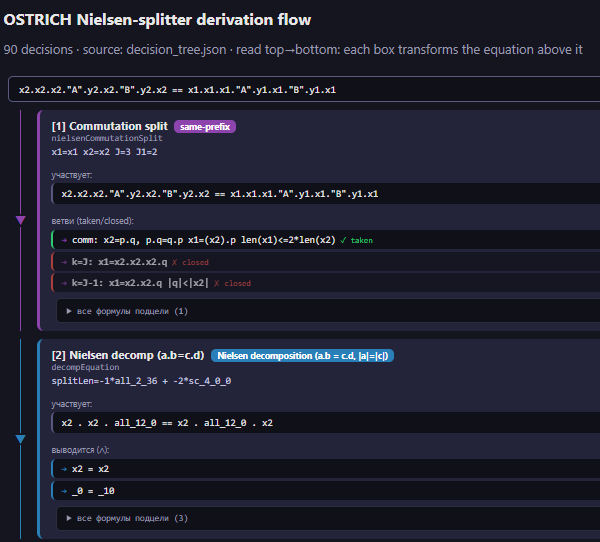
\includegraphics[width=0.72\textwidth]{screenshots/decision_tree_html.png}
\caption{Интерактивный HTML-вид дерева вывода}
\label{fig:html}
\end{figure}

\begin{figure}[h!]
\centering
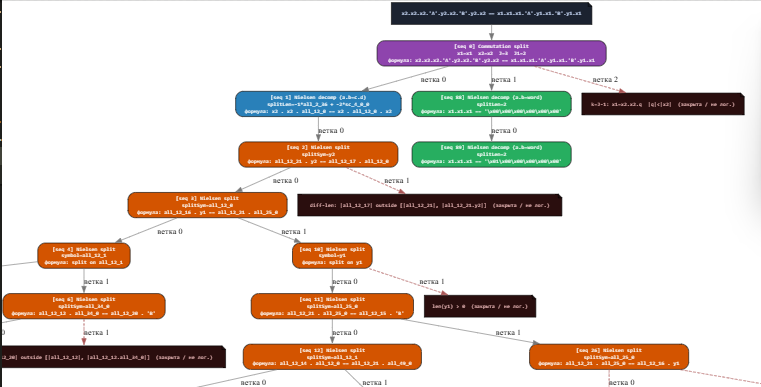
\includegraphics[width=\textwidth]{screenshots/decision_tree_graph.png}
\caption{Дерево разбора в виде графа }
\label{fig:tree}
\end{figure}

\subsection{Описание программы и руководство пользователя}
\label{sec:program}

Программа состоит из модуля-расширения решателя и набора управляющих скриптов
обвёртки (таблица~\ref{tab:modules}).

\begin{table}[h!]
\caption{Состав программных модулей}
\label{tab:modules}
\begin{tabularx}{\textwidth}{|l|X|}
\hline
Модуль & Назначение \\
\hline
\texttt{OstrichNielsenSplitter.scala} & классы коммутации (Union-Find), обнаружение
  структуры леммы, нормализация и коммутационное разбиение, логгер дерева вывода \\
\hline
\texttt{OstrichStringTheory.scala} & точка интеграции: вызовы разбиения в
  \texttt{handleGoal} \\
\hline
\texttt{ostrich\_runner.py} & запуск решателя, разбор статуса и логов \\
\hline
\texttt{gen\_smt.py} & конвертация образца в SMT-LIB (две копии уравнения) \\
\hline
\texttt{run\_patterns\_csv.py} & пакетный прогон образцов (базовая и коммутационная
  конфигурации) \\
\hline
\texttt{ambiguity\_heuristic.py} & эвристики неоднозначности (унарный, плавный,
  бинарный критерии) \\
\hline
\texttt{unambiguity\_heuristic.py} & эвристика однозначности (балансирующие разрезы) \\
\hline
\texttt{prove\_unambiguous\_by\_homomorphism.py} & перенос вердиктов по морфизмам \\
\hline
\texttt{check\_uniqueness.py} & разбор контрпримера и верификация свидетеля \\
\hline
\texttt{visualize\_decision\_tree.py} & визуализация дерева вывода (HTML, Graphviz) \\
\hline
\end{tabularx}
\end{table}

\textbf{Требования.} JDK 11 или выше, sbt, Scala~2.11; Python~3 с пакетом SymPy;
опционально --- Graphviz для рендеринга дерева вывода.
\textbf{Сборка решателя.}
\begin{Verbatim}[breaklines=true, breakanywhere=true, fontsize=\small]
java -jar sbt-launch.jar assembly
# результат: target/scala-2.11/ostrich-assembly*.jar
\end{Verbatim}

\textbf{Интерпретация результата.} В выходном CSV каждому образцу сопоставлены вердикт
(\texttt{ОДНОЗНАЧЕН} / \texttt{НЕОДНОЗНАЧЕН} / \texttt{не доказано}), сработавший
критерий или источник, свидетель ($\sigma\mid\tau$ для неоднозначности либо
балансирующий разрез для однозначности) и слово-образ. Подробное дерево вывода
решателя доступно в интерактивном файле \texttt{decision\_tree.html}.

% =====================================================================
%  РАЗДЕЛ 5. АНАЛИТИЧЕСКАЯ ЧАСТЬ  (ЗАГЛУШКА)
% =====================================================================
\section{Аналитическая часть}
\subsection{Тестирование программного обеспечения и анализ результатов}

В данном разделе представлен комплексный анализ производительности разработанного программного комплекса для определения (не)однозначности строковых паттернов. Главной целью тестирования являлась оценка эффективности предложенного гибридного конвейера, включающего в себя алгоритм быстрого эвристического поиска и специализированный строковый SMT-решатель Ostrich (О-штрих) с внедренными архитектурными улучшениями. Универсальный решатель Z3 в рамках данного исследования применялся исключительно в качестве эталонного инструмента (baseline) для верификации результатов и создания базовой линии производительности при тестировании.

\subsubsection{Верификация и оценка эвристического алгоритма}

На первом этапе оценивалась работа быстрого эвристического алгоритма, основанного на поиске разрезов и балансировок. Для проверки корректности его работы и оценки полноты покрытия был сформирован тестовый набор из 118 уникальных строковых паттернов. Результаты работы эвристики сверялись с выводами эталонного тестировщика Z3, которому выделялся лимит времени в 200 секунд на каждый паттерн.

Эвристический подход продемонстрировал себя как высокоэффективный алгоритм первичной фильтрации, работающий практически мгновенно. Детальное сравнение производительности эвристического алгоритма и эталонного решателя на сформированной выборке показало следующие результаты. Эвристика успешно разрешила 91 задачу, что составило 77\% от общего числа паттернов, в то время как Z3 за выделенное время справился с 104 паттернами (88\%). При этом критическим отличием стало время выполнения: медианное время работы эвристического метода составило менее одной миллисекунды, тогда как эталонный решатель тратил на вычисления в среднем от 1 до 9 секунд. Оба инструмента продемонстрировали высокую надежность, не допустив ни одного ложного срабатывания (False Positive). Однако эвристический подход обладает неоспоримым преимуществом в части интерпретируемости, так как для каждого успешного решения он предоставляет конкретное слово-свидетель, в то время как классический решатель выдает исключительно статус выполнимости.

Сравнение с эталонным решателем полностью подтвердило корректность предложенного метода: тестовый инструмент подтвердил неоднозначность всех 91 паттернов, решенных эвристикой, не выявив противоречий. Задачи, получившие статус «не доказано» (27 паттернов), алгоритмически передавались на следующий этап конвейера — в специализированный решатель.



\subsubsection{Оценка производительности специализированного решателя Ostrich}

Для обработки сложных структурных паттернов, не поддающихся быстрому эвристическому анализу, основным вычислительным ядром выступает строковый SMT-решатель Ostrich. Для подтверждения его эффективности было проведено нагрузочное тестирование в сравнении с базовым универсальным решателем на общей выборке из 118 паттернов.

Тестирование показало подавляющее превосходство специализированного строкового решателя в скорости обхода дерева поиска. Сравнительная характеристика решателя Ostrich и эталонного инструмента выявила ряд фундаментальных различий в их поведении. Из 118 предложенных паттернов базовый решатель Z3 успешно осилил 100 задач, тогда как Ostrich разрешил 98. Несмотря на незначительное отставание в абсолютном количестве решенных задач, медианное время выполнения на совместно решенных паттернах у Ostrich составило всего 0.74 секунды против 1.94 секунды у эталонного инструмента, что обеспечивает среднее ускорение в 2.7 раза. 

Анализ частоты превосходства по скорости показал, что Ostrich оказался быстрее в 75 случаях (63.5\% выборки), в то время как Z3 опередил оппонента лишь 39 раз. Особого внимания заслуживают нетривиальные паттерны, на которых специализированный алгоритм демонстрировал экстремальное ускорение: если максимальное зафиксированное ускорение для Z3 составило 17.5 раз, то Ostrich на задаче xAxByCyx сократил время поиска с 151 секунды до 0.12 секунды, показав превосходство в 1200 раз. Разработанный инструмент стабильно справлялся с пластом задач, вызывавших математический коллапс в универсальных алгоритмах, что визуально подтверждается логарифмическим распределением времени выполнения на соответствующем графике. 

Важным аналитическим открытием стало выявление непересекающихся «слепых зон» у обоих алгоритмов. Было зафиксировано 16 уникальных решений, доступных только базовому инструменту, которые вызвали затруднения у Ostrich. В противовес этому, 14 паттернов оказались разрешимы исключительно с помощью Ostrich, оказавшись недоступными для классической логики Z3 в рамках установленного лимита времени. Это обосновывает эффективность применения специализированных эвристик для узких классов задач.

\begin{figure}[H]
    \centering
    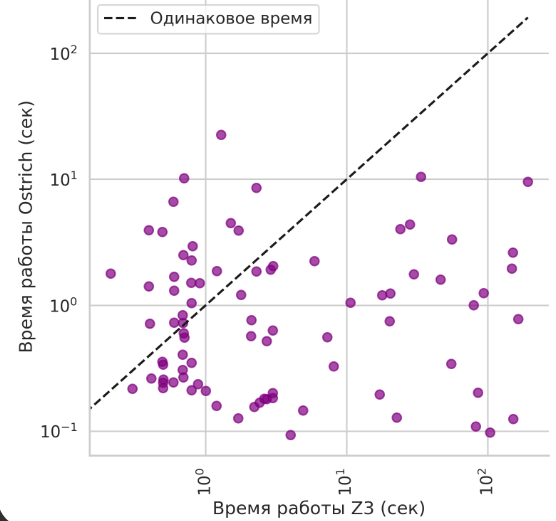
\includegraphics[width=0.8\textwidth]{z3_vs_ostrich_scatter.png}
    \caption{Сравнение времени решения: Базовый инструмент против Ostrich (логарифмическая шкала)}
    \label{fig:z3_ostrich}
\end{figure}

\subsubsection{Эффективность применения эвристики коммутативности}

В рамках тонкой настройки решателя Ostrich было исследовано влияние эвристики коммутативности на производительность поиска. Тестирование проводилось с включенным и выключенным флагом коммутативности с целью выявления накладных расходов на дополнительные проверки симметрии.

Включение данной эвристики показало себя как алгоритмически безопасная оптимизация. Базовый режим без учета коммутативности позволил решить 116 задач, тогда как включение проверок симметрии расширило это количество до 117 успешно разрешенных паттернов. Глобальное медианное время выполнения на всей тестовой выборке также продемонстрировало улучшение, снизившись с 5\.05 секунды до 4\.95 секунды.
Детальный анализ характера влияния эвристики коммутативности на процесс поиска Ostrich выявил следующее распределение. В 56 случаях, что составляет около 47\% от общего числа тестов, время работы алгоритма практически не изменилось. В 33 случаях (примерно 28\%) наблюдалось существенное ускорение работы, достигающее в пиковых значениях превосходства в 11.3 раза за счет успешного отсечения симметричных ветвей дерева решений. Естественное замедление из-за вычислительных затрат на дополнительные проверки было зафиксировано в 26 случаях (около 22\%), однако степень этого замедления оказалась некритичной. Кроме того, именно применение эвристики позволило разрешить 2 ранее недоступные задачи (около 2\% от выборки), которые при базовом прогоне уходили в таймаут. Итоговый вывод подтверждает необходимость интеграции данной эвристики в конвейер по умолчанию.

\begin{figure}[H]
    \centering
    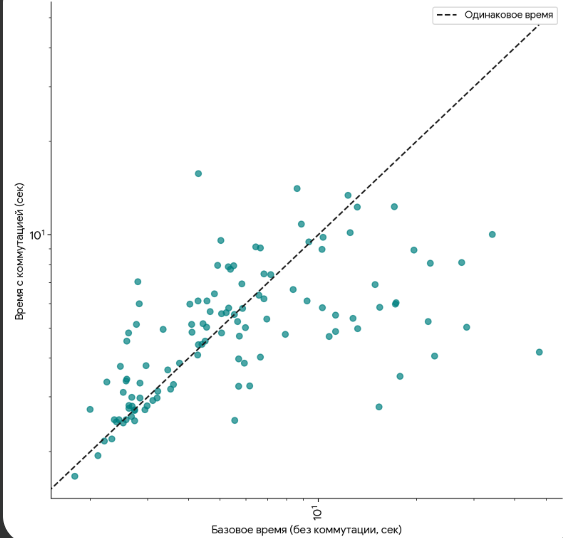
\includegraphics[width=0.8\textwidth]{commutation_scatter.png}
    \caption{Влияние эвристики коммутативности на время выполнения поиска}
    \label{fig:commutation}
\end{figure}

\subsubsection{Анализ исторической базы данных и синтез методов}

Финальным этапом аналитической работы стала проверка всего разработанного программного комплекса, включающего эвристический алгоритм, решатель Ostrich с настроенной эвристикой коммутативности и аппарат теоретических лемм, на наиболее полной исторической базе данных. Исходная база содержала 414 паттернов. Из них 179 были ранее классифицированы исследователями как неоднозначные, 14 — как однозначные, а подавляющее большинство, состоящее из 221 паттерна, имело статус строгой неопределенности и считалось алгоритмически неразрешенным.

Применение гибридного пайплайна позволило совершить существенный качественный скачок в покрытии пространства задач: из 221 ранее нерешенного паттерна конвейер смог выдать математически строгие доказательства для 56 новых случаев, что составляет 25\% от числа всех зависших задач. 

Структурная аналитика полученных решений демонстрирует четкое архитектурное разделение зон ответственности между компонентами предложенного конвейера. Математические леммы взяли на себя исключительно функцию доказательства однозначности и успешно обработали 30 тяжелых конфигураций. К этому классу относились сложные паттерны длиной от 8 символов с тремя переменными и строгими перекрестными зависимостями (например, xAxByxCxy или xAxyByxCy). Леммы оказались единственным инструментом, способным строго доказать однозначность таких структур. 

В свою очередь, решатель Ostrich и эвристический алгоритм специализировались на поиске свидетелей неodnозначности. Решатель Ostrich взял на себя обработку нелинейных вычислительно сложных паттернов, вызывавших комбинаторный взрыв при классическом переборе, и смог выявить 19 новых свидетелей неodnозначности. Эвристический алгоритм, опираясь на быстрые проверки балансировок, выявленные после оптимизации правил поиска, смог дополнительно доказать неodnозначность еще 7 паттернов. В сумме конвейер обеспечил 56 новых доказательств (30 однозначных и 26 неodnозначных).

Валидация результатов на предмет регрессий подтвердила абсолютную надежность конвейера. Все 179 паттернов, ранее доказанных как неodnозначные, и 14 однозначных паттернов были верифицированы разработанным комплексом со стопроцентной точностью. Не было зафиксировано ни одного конфликтующего вердикта по отношению к историческим данным. Данная комплексная аналитика однозначно доказывает, что предложенная гибридная архитектура позволяет нивелировать аппаратные и алгоритмические ограничения изолированных SMT-решателей, обеспечивая максимальную пробивную способность при анализе сложной строковой семантики.

% =====================================================================
%  ЗАКЛЮЧЕНИЕ
% =====================================================================
\anonsection{ЗАКЛЮЧЕНИЕ}

В настоящей работе исследованы структурные свойства строковых образцов,
содержащих повторные переменные, и разработан программный комплекс для
автоматического определения их однозначности, включающий как теоретически
обоснованные эвристики, так и расширение SMT-решателя Ostrich.

В ходе изучения теоретических основ были систематизированы алгоритмические
результаты в области уравнений в словах.

Анализ проблемы бесконечного ветвления позволил формализовать паттерн
$x^{J} y\,\Phi_1 = y^{I} x\,\Phi_2$, при котором базовый алгоритм порождает
потенциально бесконечное дерево вывода. На основе теоремы Файна--Вилфа и критерия
коммутативности Линдона--Шютценберже доказана лемма о коммутировании переменных
при удвоении, которая стала теоретическим фундаментом всех последующих оптимизаций.

Разработанное правило нормализации через классы коммутации реализовано в структуре
Union-Find с путевым сжатием и встроено в модуль \texttt{OstrichNielsenSplitter}
без изменения публичного интерфейса теории строк. Результатом стало устранение
избыточного ветвления: при включённой эвристике коммутации решатель разрешил на
один паттерн больше, чем в базовом режиме, при этом в 28\% случаев достигнуто
ускорение до 11,3 раза, а медианное время на полной выборке снизилось
с 5,05 до 4,95 секунды.

Перспективы развития проекта связаны с несколькими направлениями. Расширение
алгоритма обнаружения коммутирующих классов на уравнения с тремя и более
переменными позволит охватить паттерны, остающиеся нерешёнными в текущей
реализации. Интеграция длиновых диофантовых ограничений непосредственно в шаг
разбиения даст возможность исключать часть ветвей ещё до их раскрытия.
Наконец, автоматический синтез лемм-образцов из результатов прогонов решателя
и систематическое пополнение корпуса лемм посредством активного обучения способны
существенно ускорить обработку новых образцов за счёт накопленного теоретического
знания.

% =====================================================================
%  СПИСОК ЛИТЕРАТУРЫ
% =====================================================================
\renewcommand\refname{СПИСОК ИСПОЛЬЗОВАННЫХ ИСТОЧНИКОВ}
\clearpage
{\catcode`"\active\def"{\relax}
\addcontentsline{toc}{section}{\protect\numberline{}\refname}
\printbibliography
}

% =====================================================================
%  ПРИЛОЖЕНИЕ А. ЛИСТИНГИ
% =====================================================================
\newpage
\settocdepth{section}
\anonsection{ПРИЛОЖЕНИЕ А}
\noindent\textbf{Листинги программы}

Ниже приведены листинги реализованных методов класса
\texttt{OstrichNielsenSplitter}. Все изменения внесены в файл\\
\texttt{src/main/scala/ostrich/proofops/OstrichNielsenSplitter.scala}.


\newpage
\begin{listing}[H]
\caption{Разворачивание конкатенации в плоский список листовых термов}
\label{lst:expand}
\begin{minted}[frame=single, fontsize=\footnotesize, linenos, breaklines,
               xleftmargin=1.5em, numbersep=0.8em, breaksymbol=""]{scala}
private def expandTerm(t: LinearCombination): Seq[LinearCombination] = {
  if (strDatabase isConcrete t) {
    List(t)
  } else {
    concatPerRes.get(t) match {
      case Some(lits) if lits.size == 1 =>
        expandTerm(lits.head(0)) ++ expandTerm(lits.head(1))
      case _ =>
        List(t)
    }
  }
}

// Any non-concrete term (user variable OR intermediate concat result)
private def isUngrounded(t: LinearCombination): Boolean =
  !(strDatabase isConcrete t)

// Returns non-concrete terms that appear at least twice in the first 2 positions
private def doubledPrefix(seq: Seq[LinearCombination]): Set[LinearCombination] = {
  val pfx = seq.take(2)
  pfx.filter(t => isUngrounded(t) && pfx.count(_ == t) >= 2).toSet
}

// Returns non-concrete terms that appear at least twice in the last 2 positions
private def doubledSuffix(seq: Seq[LinearCombination]): Set[LinearCombination] = {
  val sfx = seq.takeRight(2)
  sfx.filter(t => isUngrounded(t) && sfx.count(_ == t) >= 2).toSet
}

private def prefixNonTerms(seq: Seq[LinearCombination]): Set[LinearCombination] =
  seq.take(2).filter(isUngrounded).toSet

private def suffixNonTerms(seq: Seq[LinearCombination]): Set[LinearCombination] =
  seq.takeRight(2).filter(isUngrounded).toSet
\end{minted}
\end{listing}


\newpage
\begin{listing}[H]
\caption{Предикат \texttt{isCommProxy} и его использование в \texttt{splitEquation}}
\label{lst:proxy}
\begin{minted}[frame=single, fontsize=\footnotesize, linenos, breaklines,
               xleftmargin=1.5em, numbersep=0.8em, breaksymbol=""]{scala}
private def isCommProxy(lits: Seq[Atom]): Boolean =
  lits.size == 2 && {
    val a = lits(0); val b = lits(1)
    a(0) == b(1) && a(1) == b(0)
  }

def splitEquation : Seq[Plugin.Action] = {
  val multiGroups =
    concatPerRes filter {
      case (res, lits) =>
        lits.size >= 2 && !(strDatabase isConcrete res) && !isCommProxy(lits)
    }
  // ... (остальная логика без изменений)
}
\end{minted}
\end{listing}


\newpage
\begin{listing}[H]
\caption{Метод \texttt{findEquationsWithPrefixSuffixShared}}
\label{lst:find}
\begin{minted}[frame=single, fontsize=\footnotesize, linenos, breaklines,
               xleftmargin=1.5em, numbersep=0.8em, breaksymbol=""]{scala}
def findEquationsWithPrefixSuffixShared()
    : Seq[(Atom, Atom, LinearCombination,
           Seq[LinearCombination], Seq[LinearCombination],
           Set[LinearCombination], Set[LinearCombination])] = {
  val result = new ArrayBuffer[...]

  for ((res, lits) <- concatPerRes; if lits.size >= 2) {
    for (i <- lits.indices; j <- (i + 1) until lits.size) {
      val l1  = lits(i); val l2 = lits(j)
      val lhs = expandTerm(l1(0)) ++ expandTerm(l1(1))
      val rhs = expandTerm(l2(0)) ++ expandTerm(l2(1))

      val lhsFirstIsNT = lhs.nonEmpty && isUngrounded(lhs.head)
      val rhsFirstIsNT = rhs.nonEmpty && isUngrounded(rhs.head)

      // a.a... == b.a... : doubled in one prefix, other side starts with NT
      val sharedPrefixSame =
        (if (rhsFirstIsNT) (doubledPrefix(lhs) intersect prefixNonTerms(rhs))
                             .filter(x1 => rhs.headOption.exists(_ != x1))
         else Set.empty[LinearCombination]) ++
        (if (lhsFirstIsNT) (doubledPrefix(rhs) intersect prefixNonTerms(lhs))
                             .filter(x1 => lhs.headOption.exists(_ != x1))
         else Set.empty[LinearCombination])

      // x^I... == y^J... : both sides start with DIFFERENT doubled non-terminals
      val sharedPrefixCross =
        if (sharedPrefixSame.isEmpty &&
            lhsFirstIsNT && rhsFirstIsNT &&
            doubledPrefix(lhs).nonEmpty && doubledPrefix(rhs).nonEmpty)
          doubledPrefix(lhs)
        else Set.empty[LinearCombination]

      val sharedPrefix = sharedPrefixSame ++ sharedPrefixCross
      // ... аналогично для суффиксов ...

      if (sharedPrefix.nonEmpty || sharedSuffix.nonEmpty)
        result += ((l1, l2, res, lhs, rhs, sharedPrefix, sharedSuffix))
    }
  }
  result.toSeq
}
\end{minted}
\end{listing}


\newpage
\begin{listing}[H]
\caption{Union-Find и метод \texttt{computeCommutationClasses}}
\label{lst:uf}
\begin{minted}[frame=single, fontsize=\footnotesize, linenos, breaklines,
               xleftmargin=1.5em, numbersep=0.8em, breaksymbol=""]{scala}
private def ufFind(parent: MHashMap[LinearCombination, LinearCombination],
                   x: LinearCombination): LinearCombination = {
  if (!parent.contains(x)) parent(x) = x
  if (parent(x) == x) x
  else {
    val root = ufFind(parent, parent(x))
    parent(x) = root   // путевое сжатие
    root
  }
}

private def ufUnion(parent: MHashMap[LinearCombination, LinearCombination],
                    x: LinearCombination, y: LinearCombination): Unit = {
  val rx = ufFind(parent, x); val ry = ufFind(parent, y)
  if (rx != ry) parent(rx) = ry
}

def computeCommutationClasses(): Seq[Set[LinearCombination]] = {
  val parent = new MHashMap[LinearCombination, LinearCombination]()

  for ((res, lits) <- concatPerRes; if lits.size >= 2) {
    for (i <- lits.indices; j <- (i + 1) until lits.size) {
      val lhs = expandTerm(lits(i)(0)) ++ expandTerm(lits(i)(1))
      val rhs = expandTerm(lits(j)(0)) ++ expandTerm(lits(j)(1))

      // prefix: a.a... == b.a...  =>  a commutes with b
      if (rhs.nonEmpty && isUngrounded(rhs.head))
        for (a <- doubledPrefix(lhs); if prefixNonTerms(rhs).contains(a))
          ufUnion(parent, a, rhs.head)
      if (lhs.nonEmpty && isUngrounded(lhs.head))
        for (a <- doubledPrefix(rhs); if prefixNonTerms(lhs).contains(a))
          ufUnion(parent, a, lhs.head)
      if (lhs.size == 2 && rhs.size == 2 &&
          isUngrounded(lhs.head) && isUngrounded(rhs.head) &&
          lhs(0) == rhs(1) && lhs(1) == rhs(0))
        ufUnion(parent, lhs(0), lhs(1))
    }
  }
  val groups = new MHashMap[LinearCombination, Set[LinearCombination]]()
  for (x <- parent.keys) {
    val root = ufFind(parent, x)
    groups(root) = groups.getOrElse(root, Set.empty) + x
  }
  groups.values.filter(_.size >= 2).toSeq
}
\end{minted}
\end{listing}


\newpage
\begin{listing}[H]
\caption{Методы подсчёта листовых зон и построения нормализованных форм}
\label{lst:norm_helpers}
\begin{minted}[frame=single, fontsize=\footnotesize, linenos, breaklines,
               xleftmargin=1.5em, numbersep=0.8em, breaksymbol=""]{scala}
private def prefixLenInClass(seq: Seq[LinearCombination],
                              cls: Set[LinearCombination]): Int =
  seq.indexWhere(!cls.contains(_)) match {
    case -1 => seq.length
    case n  => n
  }

private def leafZoneCountsPrefix(seq: Seq[LinearCombination],
                                  cls: Set[LinearCombination])
    : Map[LinearCombination, Int] = {
  val zone = seq.take(prefixLenInClass(seq, cls))
  zone.groupBy(identity).map { case (k, v) => k -> v.size }.withDefaultValue(0)
}

private def nonLeafTail(seq: Seq[LinearCombination],
                         cls: Set[LinearCombination]): Seq[LinearCombination] =
  seq.drop(prefixLenInClass(seq, cls))

// Returns normalized forms for both sides: (P.RL.U',  P.RR.V')
private def normalizedSeqBoth(doubledSide : Seq[LinearCombination],
                               otherSide   : Seq[LinearCombination],
                               cls         : Set[LinearCombination],
                               isSuffix    : Boolean)
    : (Seq[LinearCombination], Seq[LinearCombination]) = {
  val nuL = if (isSuffix) leafZoneCountsSuffix(doubledSide, cls)
            else           leafZoneCountsPrefix(doubledSide, cls)
  val nuR = if (isSuffix) leafZoneCountsSuffix(otherSide, cls)
            else           leafZoneCountsPrefix(otherSide, cls)
  val mz      = cls.map(z => z -> math.min(nuL(z), nuR(z))).toMap
  val sortedC = cls.toSeq.sortBy(z => (-mz(z), term2String(z)))
  val P   = sortedC.flatMap(z => Seq.fill(mz(z))(z))
  val RL  = sortedC.flatMap(z => Seq.fill(nuL(z) - mz(z))(z))
  val RR  = sortedC.flatMap(z => Seq.fill(nuR(z) - mz(z))(z))
  val uPr = if (isSuffix) nonLeafHead(doubledSide, cls) else nonLeafTail(doubledSide, cls)
  val vPr = if (isSuffix) nonLeafHead(otherSide,   cls) else nonLeafTail(otherSide,   cls)
  val normDoubled = if (isSuffix) uPr ++ RL ++ P else P ++ RL ++ uPr
  val normOther   = if (isSuffix) vPr ++ RR ++ P else P ++ RR ++ vPr
  (normDoubled, normOther)
}
\end{minted}
\end{listing}


\newpage
\begin{listing}[H]
\caption{Нормализация уравнений при известных классах коммутации}
\label{lst:normalize}
\begin{minted}[frame=single, fontsize=\footnotesize, linenos, breaklines,
               xleftmargin=1.5em, numbersep=0.8em, breaksymbol=""]{scala}
def nielsenNormalize: Seq[Plugin.Action] = {
  import TerForConvenience._
  implicit val o = order

  val eqs = findEquationsWithPrefixSuffixShared()
  if (eqs.isEmpty) return List()

  val knownClasses = computeCommutationClasses()
  val elemToClass  = (for (cls <- knownClasses; z <- cls) yield z -> cls).toMap
  val normActions  = new ArrayBuffer[Plugin.Action]

  // Priority: equations where x1, x2 already commute -> normalize without splitting
  val alreadyKnown = eqs.flatMap { case (l1e, l2e, rese, lhse, rhse, pfx, sfx) =>
    val pfxPair = pfx.headOption.flatMap { x1e =>
      val x2eOpt = if (doubledPrefix(lhse).contains(x1e)) rhse.headOption
                   else lhse.headOption
      x2eOpt.filter(x2e => elemToClass.get(x1e).exists(_.contains(x2e)))
            .map(x2e => (l1e, l2e, rese, lhse, rhse, x1e, x2e, false))
    }
    pfxPair.orElse(/* suffix analogue */ None)
  }

  if (alreadyKnown.nonEmpty) {
    for ((l1e, l2e, rese, lhse, rhse, x1e, x2e, isSfx) <- alreadyKnown) {
      val (normD, normO) = normalizedSeqBoth(lhse, rhse, Set(x1e, x2e), isSfx)
      if (normD != lhse || normO != rhse) {
        val normFormula = {
          val builder = new FormulaBuilder(goal, theory)
          if (normD.nonEmpty) builder.addConcatN(normD, rese)
          if (normO.nonEmpty) builder.addConcatN(normO, rese)
          builder.result
        }
        normActions += Plugin.AddAxiom(concatLits ++ lengthLits, normFormula, theory)
        normActions += Plugin.RemoveFacts(Conjunction.conj(List(l1e, l2e), order))
      }
    }
    return normActions.toSeq
  }
  normActions.toSeq
}
\end{minted}
\end{listing}


\newpage
\begin{listing}[H]
\caption{Трёхветвевое разбиение по коммутации}
\label{lst:commsplit}
\begin{minted}[frame=single, fontsize=\scriptsize, linenos, breaklines,
               xleftmargin=1.5em, numbersep=0.8em, breaksymbol=""]{scala}
def nielsenCommutationSplit: Seq[Plugin.Action] = {
  import TerForConvenience._
  implicit val o = order

  val eqs = findEquationsWithPrefixSuffixShared()
  if (eqs.isEmpty) return List()

  val (l1, l2, res, lhs, rhs, sharedPfx, sharedSfx) = eqs.head
  val actions = new ArrayBuffer[Plugin.Action]

  def doSplit(x1: LinearCombination, x2: LinearCombination,
              doubledSide: Seq[LinearCombination],
              otherSide:   Seq[LinearCombination],
              atomToRemove: Atom, isSuffix: Boolean): Unit = {

    val J  = if (isSuffix) otherSide.reverseIterator.takeWhile(_ == x2).length
             else          otherSide.iterator.takeWhile(_ == x2).length
    val J1 = math.max(1, J - 1)
    val commFormula = {
      val builder = new FormulaBuilder(goal, theory)
      val t = builder.newVar(StringSort)
      builder.addConjunct(_str_++(List(l(x1), l(x2), l(t))))
      builder.addConjunct(_str_++(List(l(x2), l(x1), l(t))))
      if (J1 > 0)
        for (lenX1 <- lengthMap.get(x1); lenX2 <- lengthMap.get(x2))
          builder.addConjunct(
            sum(List((IdealInt(J1), l(lenX2)), (IdealInt.MINUS_ONE, l(lenX1)))) >= 0)
      builder.result
    }
    val caseJFormula = {
      val builder = new FormulaBuilder(goal, theory)
      val q = builder.newVar(StringSort)
      if (isSuffix) builder.addConcatN(q +: Seq.fill(J)(x2 : Term), x1)
      else          builder.addConcatN(Seq.fill(J)(x2 : Term) :+ q,  x1)
      builder.result
    }
    val caseJ1Formula = {
      val builder = new FormulaBuilder(goal, theory)
      val q = builder.newVar(StringSort)
      if (isSuffix) builder.addConcatN(q +: Seq.fill(J1)(x2 : Term), x1)
      else          builder.addConcatN(Seq.fill(J1)(x2 : Term) :+ q,  x1)
      builder.result
    }
    val doubledAtom: Atom = if (atomToRemove eq l2) l1 else l2
    val removeBoth  = Conjunction.conj(List(atomToRemove, doubledAtom), order)
    val removeOther = Conjunction.conj(atomToRemove, order)
    actions += Plugin.AxiomSplit(
      concatLits ++ lengthLits,
      List(
        (commFormula,   List(Plugin.RemoveFacts(removeBoth))),
        (caseJFormula,  List(Plugin.RemoveFacts(removeOther))),
        (caseJ1Formula, List(Plugin.RemoveFacts(removeOther)))
      ),
      theory
    )
  }
}
\end{minted}
\end{listing}

\end{document}
